% Options for packages loaded elsewhere
\PassOptionsToPackage{unicode}{hyperref}
\PassOptionsToPackage{hyphens}{url}
%
\documentclass[
  spanish,
]{book}
\usepackage{lmodern}
\usepackage{amsmath}
\usepackage{ifxetex,ifluatex}
\ifnum 0\ifxetex 1\fi\ifluatex 1\fi=0 % if pdftex
  \usepackage[T1]{fontenc}
  \usepackage[utf8]{inputenc}
  \usepackage{textcomp} % provide euro and other symbols
  \usepackage{amssymb}
\else % if luatex or xetex
  \usepackage{unicode-math}
  \defaultfontfeatures{Scale=MatchLowercase}
  \defaultfontfeatures[\rmfamily]{Ligatures=TeX,Scale=1}
\fi
% Use upquote if available, for straight quotes in verbatim environments
\IfFileExists{upquote.sty}{\usepackage{upquote}}{}
\IfFileExists{microtype.sty}{% use microtype if available
  \usepackage[]{microtype}
  \UseMicrotypeSet[protrusion]{basicmath} % disable protrusion for tt fonts
}{}
\makeatletter
\@ifundefined{KOMAClassName}{% if non-KOMA class
  \IfFileExists{parskip.sty}{%
    \usepackage{parskip}
  }{% else
    \setlength{\parindent}{0pt}
    \setlength{\parskip}{6pt plus 2pt minus 1pt}}
}{% if KOMA class
  \KOMAoptions{parskip=half}}
\makeatother
\usepackage{xcolor}
\IfFileExists{xurl.sty}{\usepackage{xurl}}{} % add URL line breaks if available
\IfFileExists{bookmark.sty}{\usepackage{bookmark}}{\usepackage{hyperref}}
\hypersetup{
  pdftitle={Manual de uso de scritps de automatización de tabulados de Registros Administrativos de Seguridad Pública y Justicia},
  pdfauthor={Daniel M. Giménez},
  pdflang={es-ES},
  hidelinks,
  pdfcreator={LaTeX via pandoc}}
\urlstyle{same} % disable monospaced font for URLs
\usepackage{color}
\usepackage{fancyvrb}
\newcommand{\VerbBar}{|}
\newcommand{\VERB}{\Verb[commandchars=\\\{\}]}
\DefineVerbatimEnvironment{Highlighting}{Verbatim}{commandchars=\\\{\}}
% Add ',fontsize=\small' for more characters per line
\usepackage{framed}
\definecolor{shadecolor}{RGB}{248,248,248}
\newenvironment{Shaded}{\begin{snugshade}}{\end{snugshade}}
\newcommand{\AlertTok}[1]{\textcolor[rgb]{0.94,0.16,0.16}{#1}}
\newcommand{\AnnotationTok}[1]{\textcolor[rgb]{0.56,0.35,0.01}{\textbf{\textit{#1}}}}
\newcommand{\AttributeTok}[1]{\textcolor[rgb]{0.77,0.63,0.00}{#1}}
\newcommand{\BaseNTok}[1]{\textcolor[rgb]{0.00,0.00,0.81}{#1}}
\newcommand{\BuiltInTok}[1]{#1}
\newcommand{\CharTok}[1]{\textcolor[rgb]{0.31,0.60,0.02}{#1}}
\newcommand{\CommentTok}[1]{\textcolor[rgb]{0.56,0.35,0.01}{\textit{#1}}}
\newcommand{\CommentVarTok}[1]{\textcolor[rgb]{0.56,0.35,0.01}{\textbf{\textit{#1}}}}
\newcommand{\ConstantTok}[1]{\textcolor[rgb]{0.00,0.00,0.00}{#1}}
\newcommand{\ControlFlowTok}[1]{\textcolor[rgb]{0.13,0.29,0.53}{\textbf{#1}}}
\newcommand{\DataTypeTok}[1]{\textcolor[rgb]{0.13,0.29,0.53}{#1}}
\newcommand{\DecValTok}[1]{\textcolor[rgb]{0.00,0.00,0.81}{#1}}
\newcommand{\DocumentationTok}[1]{\textcolor[rgb]{0.56,0.35,0.01}{\textbf{\textit{#1}}}}
\newcommand{\ErrorTok}[1]{\textcolor[rgb]{0.64,0.00,0.00}{\textbf{#1}}}
\newcommand{\ExtensionTok}[1]{#1}
\newcommand{\FloatTok}[1]{\textcolor[rgb]{0.00,0.00,0.81}{#1}}
\newcommand{\FunctionTok}[1]{\textcolor[rgb]{0.00,0.00,0.00}{#1}}
\newcommand{\ImportTok}[1]{#1}
\newcommand{\InformationTok}[1]{\textcolor[rgb]{0.56,0.35,0.01}{\textbf{\textit{#1}}}}
\newcommand{\KeywordTok}[1]{\textcolor[rgb]{0.13,0.29,0.53}{\textbf{#1}}}
\newcommand{\NormalTok}[1]{#1}
\newcommand{\OperatorTok}[1]{\textcolor[rgb]{0.81,0.36,0.00}{\textbf{#1}}}
\newcommand{\OtherTok}[1]{\textcolor[rgb]{0.56,0.35,0.01}{#1}}
\newcommand{\PreprocessorTok}[1]{\textcolor[rgb]{0.56,0.35,0.01}{\textit{#1}}}
\newcommand{\RegionMarkerTok}[1]{#1}
\newcommand{\SpecialCharTok}[1]{\textcolor[rgb]{0.00,0.00,0.00}{#1}}
\newcommand{\SpecialStringTok}[1]{\textcolor[rgb]{0.31,0.60,0.02}{#1}}
\newcommand{\StringTok}[1]{\textcolor[rgb]{0.31,0.60,0.02}{#1}}
\newcommand{\VariableTok}[1]{\textcolor[rgb]{0.00,0.00,0.00}{#1}}
\newcommand{\VerbatimStringTok}[1]{\textcolor[rgb]{0.31,0.60,0.02}{#1}}
\newcommand{\WarningTok}[1]{\textcolor[rgb]{0.56,0.35,0.01}{\textbf{\textit{#1}}}}
\usepackage{longtable,booktabs}
\usepackage{calc} % for calculating minipage widths
% Correct order of tables after \paragraph or \subparagraph
\usepackage{etoolbox}
\makeatletter
\patchcmd\longtable{\par}{\if@noskipsec\mbox{}\fi\par}{}{}
\makeatother
% Allow footnotes in longtable head/foot
\IfFileExists{footnotehyper.sty}{\usepackage{footnotehyper}}{\usepackage{footnote}}
\makesavenoteenv{longtable}
\usepackage{graphicx}
\makeatletter
\def\maxwidth{\ifdim\Gin@nat@width>\linewidth\linewidth\else\Gin@nat@width\fi}
\def\maxheight{\ifdim\Gin@nat@height>\textheight\textheight\else\Gin@nat@height\fi}
\makeatother
% Scale images if necessary, so that they will not overflow the page
% margins by default, and it is still possible to overwrite the defaults
% using explicit options in \includegraphics[width, height, ...]{}
\setkeys{Gin}{width=\maxwidth,height=\maxheight,keepaspectratio}
% Set default figure placement to htbp
\makeatletter
\def\fps@figure{htbp}
\makeatother
\setlength{\emergencystretch}{3em} % prevent overfull lines
\providecommand{\tightlist}{%
  \setlength{\itemsep}{0pt}\setlength{\parskip}{0pt}}
\setcounter{secnumdepth}{5}
\usepackage{booktabs}
\ifxetex
  % Load polyglossia as late as possible: uses bidi with RTL langages (e.g. Hebrew, Arabic)
  \usepackage{polyglossia}
  \setmainlanguage[]{spanish}
\else
  \usepackage[shorthands=off,main=spanish]{babel}
\fi
\ifluatex
  \usepackage{selnolig}  % disable illegal ligatures
\fi
\usepackage[]{natbib}
\bibliographystyle{apalike}

\title{Manual de uso de scritps de automatización de tabulados de Registros Administrativos de Seguridad Pública y Justicia}
\author{Daniel M. Giménez}
\date{2021-02-01}

\begin{document}
\maketitle

{
\setcounter{tocdepth}{1}
\tableofcontents
}
\hypertarget{part-portada}{%
\part*{PORTADA}\label{part-portada}}
\addcontentsline{toc}{part}{PORTADA}

\begin{center}\rule{0.5\linewidth}{0.5pt}\end{center}

\hypertarget{presentaciuxf3n}{%
\chapter*{Presentación}\label{presentaciuxf3n}}
\addcontentsline{toc}{chapter}{Presentación}

Como parte de la política de mejoramiento continuo que implementa desde 2014, la Unidad de Seguridad Pública y Justicia del Subdepartamento de Condiciones de Vida del INE inició en el transcurso del año 2020 la automatización de los procesos de generación de tabulados de los Informes Anuales de Estadísticas Policiales y de Estadísticas Judiciales. Dicha automatización se ha realizado a través de programación estadística en el software \emph{R Project for Statistical Computing} (sólo R de aquí en adelante).

El resultado de la automatización es un sistema de \emph{scripts} que transforma las bases de datos de las tres fuentes administrativas con las que trabaja la Unidad (Policía de Investigaciones, Carabineros de Chile y Poder Judicial) en los cuadros en formato Excel que se publican junto a los informes anuales arriba mencionados.

Para que el sistema realice esto, se requiere preparar con precisión los insumos que toman los \emph{scripts} para generar los tabulados. ``Precisión'' acá significa ``cumpliendo procedimientos muy específicos y aplicándoles de forma estricta ciertos formatos y estructuras''. De lo contrario, el script puede arrojar errores y/o no comportarse como ha sido programado. En otras palabras, el procesamiento automatizado es «frágil»: cualquier incumplimiento, por más mínimo que sea, con los formatos, estructuras de bases de datos o los procedimientos exigidos por los \emph{scripts} arrojará error o resultados no esperados.

El objetivo del presente documento es detallar los procedimientos, los formatos y las estructuras que se deben seguir, respetar y/o aplicar para que los \emph{scripts} de automatización funcionen correctamente, cumplan su propósito y entreguen los tabulados validados para los que han sido programados. Es, por lo tanto, un \textbf{\emph{manual para generar de forma automatizada los tabulados y las validaciones de Registros Administrativos (RRAA) usando el script específicamente programado para esos propósitos}}.

A grandes rasgos, este Manual tiene cuatro objetivos:

\begin{itemize}
\item
  Guiar con instrucciones detalladas el proceso de generación de los insumos necesarios para la producción de los tabulados y su validación;
\item
  Explicar cómo se inician y ejecutan los procesos de generación automatizada de tabulados y validaciones contenidos en los \emph{scripts};
\item
  Mostrar de forma genérica la estructura de archivos de los \emph{scripts} para que cualquier persona con conocimiento de R pueda modificarlos cuando sea necesario generar nuevos cuadros o cambiarlos de posición en los libros finales de Excel;
\item
  Entregar criterios generales para el mantenimientos del código y para identificar y corregir potenciales errores que pudieran producirse en el procesamiento de bases de datos en las próximas versiones de los Informes Anuales.
\end{itemize}

Todas las instrucciones y definiciones de este Manual suponen que se han seguido y cumplido los protocolos establecidos en el \textbf{\emph{Manual de Protocolos de Automatización}}. Ahí se encuentran detalladas no sólo las condiciones mínimas que deben cumplirse para iniciar tareas de automatizado de bases de datos de RRAA, sino también los criterios y estándares mínimos a los que deben ajustarse los datos, los archivos auxiliares, el código y los \emph{scripts} de automatización.

De todas formas, en la redacción del presente Manual se ha tenido especial cuidado en explicar en qué consiste cada procedimiento necesario para que el sistema de \emph{scripts} funcione. La idea no es ejecutar de forma mecánica las instrucciones acá contenidas. Al contrario. Es ejecutarlas con consciencia de lo que hacen y por qué se realizan esas operaciones en particular y de la forma específica en que se realizan. Sólo así se podrá tener control sobre su funcionamiento.

El Manual consta de tres partes. La primera está dedicada a explicar detalladamente cómo se ha concebido y desarrollado el \emph{script}; es el marco necesario para comprender lo que se debe hacer (y por qué) para lograr los resultados buscados con su ejecución.

La segunda parte detalla cómo se generan y preparan los insumos necesarios que alimentarán a los \emph{scripts} para que produzcan los tabulados: las bases de datos y los archivos auxiliares.

La tercera parte está dedicada a describir cómo funciona y opera el conjunto de los \emph{scripts} para que se puedan intervenir en caso de que sea necesario.

\hypertarget{part-primera-parte-el-sistema-de-scripts}{%
\part*{PRIMERA PARTE: EL SISTEMA DE SCRIPTS}\label{part-primera-parte-el-sistema-de-scripts}}
\addcontentsline{toc}{part}{PRIMERA PARTE: EL SISTEMA DE SCRIPTS}

\hypertarget{presentaciuxf3n-de-la-primera-parte}{%
\chapter*{Presentación de la primera parte}\label{presentaciuxf3n-de-la-primera-parte}}
\addcontentsline{toc}{chapter}{Presentación de la primera parte}

Para el desarrollo del sistema de \emph{scripts} de automatización se han tomado importantes decisiones orientadas a facilitar su funcionamiento, alimentación y mantenimiento. Para poder operar con él, es de mucha ayuda conocer la lógica con la que se ha concebido. El primer capítulo de esta primera parte tiene ese propósito: explicar el funcionamiento general del sistema de \emph{scripts} y por qué se desarrolló así.

El segundo capítulo expone las convenciones generales usadas en los \emph{scripts} y las que se aplican en el presente manual.

\hypertarget{la-perspectiva-de-automatizaciuxf3n-aplicada}{%
\chapter{La perspectiva de automatización aplicada}\label{la-perspectiva-de-automatizaciuxf3n-aplicada}}

\hypertarget{la-soluciuxf3n-de-programadora}{%
\section{La solución de ``programador/a''}\label{la-soluciuxf3n-de-programadora}}

Las soluciones computacionales aplican la lógica del i/o: reciben un input, lo procesan con un programa y entregan un output, el programado. En gran medida, es la lógica que aplican las soluciones de automatización en todas partes, desde aplicaciones simples en sistemas operativos Automator en MacOS, por ejemplo) hasta soluciones complejas en la nube.

Si aplicamos de forma estricta esta lógica a la automatización de la producción estadística (que es lo que hace el sistema \emph{scripts} para el cual se escribió este manual: producción estadística), cualquier solución automatizada debiera tomar bases de datos (input) y mediante un programa (un conjunto de códigos) generar tabulados o gráficos (output).

A grandes rasgos, esa fue la primera solución que se pensó para este sistema de \emph{scripts}. Sin embargo, resultó una solución limitada en muy poco tiempo. Para generar los tabulados que publica la Unidad de Seguridad Pública y Justicia (SPyJ), además de las bases de datos, se requieren títulos, notas al pie y otros elementos de información adicionales (fuentes, notas aclaratorias, etc). Ninguno de esos elementos, sin embargo, viene en las bases de datos. Es necesario agregárselos en alguna fase del procesamiento. Y si seguimos la lógica habitual i/o de las soluciones computacionales, la agregación tendría que hacerse en o a través del código del programa, en los \emph{scripts} mismos.

Esta solución es inadecuada y poco óptima por tres motivos:

\begin{enumerate}
\def\labelenumi{\arabic{enumi}.}
\item
  Es un formato poco flexible, de difícil adaptación a cambios en los inputs o en los outputs. Si se requiriera agregar una nota a un tabulado, por ejemplo, sería necesario intervenir directamente el código de algún \emph{scritpt}. Y puesto que toda intervención en el código supone un riesgo de romperlo o alterar su funcionamiento, el balance final del costo/beneficio de agregar una simple nota a un cuadro es poco ventajoso.
\item
  Para hacer cualquier ajuste mínimo en un cuadro y, por lo tanto, para intervenir el código, es necesario tener conocimiento del lenguaje de programación; en este caso, de R. Pero no sólo eso: dado que se trata de un proyecto complejo, también es necesario estar familiarizado/a con el sistema de scripts y su estructura. Demasiada exigencia para el simple añadido de una nota al pie.
\item
  Esta solución demandaría una mantención del código más intensiva y regular, pues cualquier variación en los inputs o outputs supondría hacer ajustes o actualizaciones en los \emph{scripts}.
\end{enumerate}

A la larga, esta forma de abordar, pensar y desarrollar una solución automatizada está hecha a medida de programadores/as. Y no de cualquier programador/a: de un/a que conozca con detalle este código.

\hypertarget{la-soluciuxf3n-de-usuarioa-de-excel}{%
\section{La solución de usuario/a de Excel}\label{la-soluciuxf3n-de-usuarioa-de-excel}}

Las limitaciones de la solución anterior son especialmente significativas en el caso de los tabulados de SPyJ. Al menos dos son las más importantes:

\begin{enumerate}
\def\labelenumi{\arabic{enumi}.}
\item
  Las bases de datos o los tabulados que se generan con ellas sufren modificaciones año a año. No necesariamente son modificaciones estructurales o grandes, pero son modificaciones al fin del cabo. Siendo la mayoría de ellas muy pequeñas, como la agregación de la nota al pie descrita en la sección anterior, no sale a cuenta intervenir los \emph{scripts}.
\item
  El presente sistema de \emph{scripts} no será usado ni operado por programadores/as ni mucho menos por las personas responsables de crearlo y programarlo. Será operado por profesionales que trabajan con las estadísticas pero no con programación. Aplicar la solución i/o descrita en la sección anterior supondría generar una alta dependencia de programadores/as en R para actualizar o adecuar el código.
\end{enumerate}

Para superar ambas limitaciones, se ideó un mecanismo que a) evitará intervenir el código para actualizar y ajustar los elementos que se añaden a los cuadros; b) que pudiera ser usado y manipulado por personas que no tengan conocimientos avanzados ni de R ni de la estructura y funcionamiento del código de los \emph{scripts}.

El mecanismo es introducir los datos complementarios a través de un archivo Excel distinto a las bases de datos que se usan para generar los tabulados. A falta de mejor concepto, se lo bautizó con el nombre de ``diccionario''. En el Capítulo 4 se explica con detalle la estructura y contenidos de este archivo. Por el momento, basta con saber que los \emph{scripts} han sido desarrollados para que tomen de este archivo la información necesaria para:

\begin{enumerate}
\def\labelenumi{\arabic{enumi}.}
\item
  Agregar notas, títulos y otros textos a los cuadros;
\item
  Tomar las glosas o etiquetas de categorías que no procede o conviene tomar directamente de las bases de datos;
\item
  Datos de años anteriores para cuadros de series temporales.
\end{enumerate}

Gracias al diccionario, la actualización de los distintos elementos de los cuadros requiere ya no saber programar en R, sino solamente un conocimiento funcional de Excel.

\hypertarget{el-control-del-flujo}{%
\section{El control del flujo}\label{el-control-del-flujo}}

Adicionalmente, se le ha asignado al archivo del diccionario la tarea de controlar el flujo de los \emph{scripts}. En el Capítulo 4 se detalla cómo hace eso.

\hypertarget{reglas-de-formato-y-convenciones-del-manual}{%
\chapter{Reglas de formato y convenciones del Manual}\label{reglas-de-formato-y-convenciones-del-manual}}

\hypertarget{formatos-para-los-scripts}{%
\section{Formatos para los scripts}\label{formatos-para-los-scripts}}

Para el funcionamiento de los \emph{scripts} se han aplicado algunos formatos a varios elementos que se recomienda seguir y replicar en el futuro. No hay nada que indique que no seguirlos pudiera generar algún error o problema, pero mejor evitar cualquier riesgo.

Los formatos aplicados fueron los siguientes:

\begin{enumerate}
\def\labelenumi{\alph{enumi})}
\item
  \textbf{nombres de archivos}: todos los nombres de archivos se escriben sin espacios y, salvo excepciones, en minúsculas. Los espacios ha sido sustituidos por guiones bajos. Y mayúsculas se ocupan en circunstancias muy particulares, como, por ejemplo, en el identificador de la unidad institucional al que corresponde un archivo. El diccionario, por ejemplo, ha sido bautizado con el siguiente nombre: \texttt{diccionarios\_SPyJ\_2019.xlsx}.
\item
  \textbf{extensión de los archivos}: las extensiones de los archivos se pueden escribir indistintamente en minúsculas o mayúsculas: xlsx o XLSX. Para la mayor parte de los casos, el \emph{script} puede interpretar ambas formas. Así no exige romper con algunos formatos habituales de escribir extensiones: .RData, .RDS, .R, etc. De todas formas, siempre que exista la posibilidad, es preferible usar minúsculas.
\item
  \textbf{la fuente}: en los archivos de los \emph{scripts} y en algunos campos del diccionario se agrega la fuente al final del nombre. Por ejemplo, el archivo de tabulados de PDI se llama \texttt{tabs\_pdi.R}. Esto debe manternerse obligatoriamente en las columnas del diccionario. No puede suprimirse.
\item
  \textbf{nombres de columnas}: los nombres de las columnas de las bases de datos se escriben siempre sin espacios y en minúsculas. Si es necesario separar dos palabras, se usa el guión bajo. Es recomendable evitar signos extraños, desde tildes hasta la ñ. Números, letras y guiones bajos bastan y sobran.
\end{enumerate}

\hypertarget{formatos_manual}{%
\section{Formatos de codigo en este manual}\label{formatos_manual}}

En algunas partes de este manual se ha incorporado código de R para indicar qué operaciones deben realizarse y cómo. Se han aplicado los siguientes formatos:

\begin{enumerate}
\def\labelenumi{\alph{enumi})}
\tightlist
\item
  \textbf{nombres de objetos u otros elementos}: los nombres o las partes del código que pueden y deben ser sustituidas con nombres o textos se escriben entre signos de mayor (\textless) y menor (\textgreater). Cada vez que aparezca un contenido así, entonces, se sustituye por el contenido que corresponda. Ejemplo: \texttt{\textless{}objeto\textgreater{}\ \textless{}-\ read.delim("\textless{}ruta\ al\ archivo\textgreater{}",\ sep\ =\ ";")}
\end{enumerate}

En ese caso, los signos mayor y menor indican que en el nombre del objeto y la ruta al archivo deben reemplazarse los textos con el contenido que corresponda.

\begin{enumerate}
\def\labelenumi{\alph{enumi})}
\setcounter{enumi}{1}
\tightlist
\item
  \textbf{nombre de paquetes}: cuando en el manual se usan funciones de paquetes distintos a R base, se agregan sus nombres antes de la función seguido de doble dos puntos. Así: \texttt{paquete::función()}. De esta forma, si algún pedazo de código del manual genera un error de ``función no encontrada'', ya se sabe qué paquete se debe instalar para que funcione. La instalación se hace con la siguiente función: \texttt{install.packages("\textless{}nombre\ del\ paquete\textgreater{}")}.
\end{enumerate}

\hypertarget{part-segunda-parte-la-fase-manual}{%
\part*{SEGUNDA PARTE: LA FASE MANUAL}\label{part-segunda-parte-la-fase-manual}}
\addcontentsline{toc}{part}{SEGUNDA PARTE: LA FASE MANUAL}

\hypertarget{presentaciuxf3n-de-la-segunda-parte}{%
\chapter*{Presentación de la segunda parte}\label{presentaciuxf3n-de-la-segunda-parte}}
\addcontentsline{toc}{chapter}{Presentación de la segunda parte}

Un proceso de automatización tiene el propósito de asignar a un programa o factores de trabajo no humano el trabajo que, sin dicha automatización, sería realizado por seres humanos. En ningún trabajo automatizado, sin embargo, es posible eliminar por completo el trabajo humano. Cualquiera sea el proceso automatizado (desde la construcción de motores de aviones supersónicos hasta la producción estadística), dicho trabajo es necesario al menos para la preparación de los insumos que alimentan la automatización.

Aunque en el lenguaje cotidiano suele llamarse, equivocadamente, ``fase manual'' a esta fase de trabajo humano, no todo trabajo humano destinado a preparar los insumos para un procesamiento automatizado es ``manual''. Sin embargo, para evitar confusiones, y dado que ya se encuentra instalado, se usará dicho término en el presente manual; también se usará indistintamente el término ``fase de preparación''.

La ``fase manual'' o ``fase de preparación'' de un proceso de automatización, entonces, consiste en preparar, mediante trabajo humano, los insumos necesarios que alimentan a dicho proceso. Y para el éxito de la automatización es fundamental que la preparación de los insumos se realice de forma rigurosa, precisa y siguiendo protocolos y reglas de forma estricta.

Esta segunda parte del Manual tiene el propósito de describir los insumos fundamentales que la automatización de tabulados requiere y explicar detalladamente las reglas y protocolos que deben cumplirse en toda esta fase de preparación para que el código genere los resultados esperados y no arroje errores.

Los insumos necesarios para que se ejecute el script son dos: las bases de datos y un archivo en Excel que para efectos de la automatización en SPyJ se ha llamado ``diccionario''. Adicionalmente y de forma opcional, si también se requiere validar los tabulados, es necesario generar un archivo validador por cada fuente. Pero el sistema de \emph{scripts} puede ejecutarse sin él; para que funcione y genere resultados, son requisitos las bases de datos y el diccionario.

Las bases de datos son el conjunto de la información recibida de las fuentes administrativas y de cuyo procesamiento se obtienen las estadísticas que publica la unidad. Puesto que cada fuente tiene formatos, codificaciones y estructuras de datos distintos, parte importante de la fase de preparación está dedicada a la estandarización de bases de datos para que los \emph{scripts} las entiendan y las procesen. El primer capítulo de esta segunda parte está dedicado a detallar las estructuras de bases de datos, los formatos de la información y las precauciones generales que deben tenerse para alimentar los \emph{scripts} con esas bases.

El diccionario, por su parte, es un archivo Excel que cumple una doble función. Por un lado, a través de su contenido es posible controlar el flujo del sistema de \emph{scripts} sin necesidad de intervenir su código. Por otro lado, el diccionario contiene toda la información auxiliar, no contenida en las bases de datos, que utilizan los \emph{scripts} para generar tabulados y validarlos. Cualquier información que se requiera agregar a los cuadros y a la validación, se ingresa a través de este archivo Excel. Gracias a ello, tan sólo con conocimiento de Excel es posible ajustar los detalles de los tabulados, sin necesidad de intervenir el código en R. Por ejemplo, para incorporar una nota o un título a un cuadro, simplemente se la incorpora en este archivo de diccionario, y el script la añade automáticamente. Para que haga esta operación correctamente, se requiere ingresar la información de forma muy cuidadosa, precisa y rigurosa. El segundo capítulo de esta segunda parte explica la estructura de este archivo ``diccionario'' y cómo debe ingresarse la información en él para que pueda ser incorporada de forma correcta por los \emph{scripts}.

Finalmente, el validador es un archivo en formato Excel que contiene los datos de los tabulados que se espera produzca el sistema de \emph{scripts}. Se le ordena al script que valide los resultados a través del diccionario. El tercer capítulo de esta segunda parte explica cómo se realiza ese proceso.

\hypertarget{las-bases-de-datos}{%
\chapter{Las bases de datos}\label{las-bases-de-datos}}

Como se mencionaba, cada fuente administrativa remite la información necesaria para que el INE produzca sus estadísticas en formatos propios. No ha habido un proceso de estandarización la información pedida ni en la forma de remitirla, como se establece en el \textbf{Manual de Protocolos de Automatización}. Y esto genera un importante problema para un código de automatización que sea capaz de generar productos a partir de dos o más fuentes administrativas: debe ser capaz de procesar información con distintas estructuras y formatos.

Hay dos alternativas para lidiar con este problema. La primera es evitar la manipulación de las bases de datos y ajustar el código de los \emph{scripts} de automatización a cada formato distinto de cada base de datos distinta. La segunda alternativa es intervenir y modificar manualmente las bases de datos para estandarizarlas; así, un único código general es capaz de generar cualquier tabulado.

Las dos alternativas tienen ventajas y desventajas. En el primer caso, se mantendría la integridad de los datos; se procesarían tal y como han sido remitidos por la fuente. Pero eso a costo de escribir un código muy largo e ineficiente para que pueda hacerse cargo de problemas y formatos específicos y puntuales de cada base de datos. La Corporación Adminsitrativa del Poder Judicial, por ejemplo, remite 18 bases de datos con al menos 8 estructuras y formatos distintos. Para que el \emph{script} respectivo pudiera procesar todos esas distintas variantes, tendría que contener un código largo y más lento. Esta solución, además, tendría un limitación importante: si los próximos años se produce alguna modificación de la estructura o de los formatos de los datos remitidos por la fuente administrativa, sería necesario intervenir nuevamente el \emph{script} para agregar o adaptar código a las nuevas estructuras o formatos.

La segunda solución, la intervención manual en las bases, permite dos cosas fundamentales: por un lado, escribir un único código con funciones para procesar todos los tipos y formatos de bases de datos; y, por el otro lado, permite reducir las posibilidad de intervenir los contenidos y las funciones del script en caso de que en futuras versiones de los datos se produzca algún cambio de estructura o formato. Y hay una ventaja adicional: interviniendo manualmente las bases para adaptarlas al código del sistema de \emph{scripts}, es posible usar este mismo script para desarrollar código que permita generar tabulados de fuentes distintas a las contempladas inicialmente en el desarrollo del código. En otros términos, adoptando esta segunda solución, este mismo sistema de \emph{scripts} puede usarse para automatizar la generación de tabulados de fuentes distintas a las que alimentan las estadísticas de SPyJ.

Dos son las desventajas de esta segunda solución. La primera: exige alterar los datos de origen. La segunda: no es posible adelantarse a todas las variaciones posibles que incluirán las bases de datos en el futuro. Por lo tanto, la estandarización tiene un techo, y es altamente improbable que no sea necesario ajustar el código de los \emph{scripts} cada año para que pueda procesar nuevos datos. Las potenciales intervenciones al código con esta solución, sin embargo, son menores en cantidad y profundidad que con la primera solución.

En vista de las ventajas y desventajas de las dos posibles soluciones, para el sistema de \emph{scripts} de automatización de tabulados y validaciones de SPyJ se ha optado por una combinación de ambas. Se estandarizan elementos generales de las bases de datos, en particular nombres y formatos de variables y algunos formatos de datos. Pero, a la vez, se evita alterar el contenido fundamental de cada base de datos. Las funciones del script han sido escritas para aprovechar lo que se puede estandarizar y también para que tengan la flexibilidad suficiente para procesar diversas estructuras y formatos.

La solución híbrida adoptada es eficaz, pero exige precisión en la intervención manual de las bases de datos para ajustarlas al código de los \emph{scripts}. ¨El presente capítulo detalla las principales instrucciones para realizar ese proceso.

Estas instrucciones deben seguirse de forma estricta; salvo por el formato de los archivos de las bases de datos, no hay alternativas posibles entre las que elegir en el tratamiento y manipulación de las bases.

\hypertarget{los-formatos-admitidos}{%
\section{Los formatos admitidos}\label{los-formatos-admitidos}}

Los \emph{scripts} admiten tres formatos de bases de datos: csv, xlsx y rds. Los dos primeros, csv y xlsx, son de uso masivo y relativamente estandarizado. Por esta razón, es altamente probable que las fuentes administrativas remitan sus datos en alguno de ellos.

También es probable que para bases de datos de más de 1.000.000 de casos, algunas fuentes administrativas usen el formato binario de Excel (xlsb). Este formato, sin embargo, se carga de forma algo errática en R; hasta donde se han testeado para el desarrollo del presente sistema de \emph{scripts}, ninguna de las librerías disponibles para su tratamiento es capaz de cargar de forma óptima la totalidad de archivos xlsb con los que se ha probado. Por esta razón, se ha descartado en el script el soporte a la carga de datos en ese formato. Para que pueda procesar un archivo remitido por las fuentes administrativas en este formato, es necesario transformarlo antes a formato csv a través de Excel.

Los \emph{scripts} tampoco tienen soporte para archivos xls. Si la fuente remite alguno en este formato, debe convertirse a formato xlsx a través de Excel.

El rds, por su parte, es un formato interno de R. Es el más eficaz en velocidad de procesamiento, consumo de memoria RAM y espacio ocupado en disco. Sin embargo, por ser un formato interno de R, es altamente improbable que las fuentes administrativas lo ocupen para remitir la información al INE. Salvo por R y Python (con el módulo \texttt{pyreadr}), ningún otro programa es capaz de guardar o leer datos en este formato. Para generar el archivo, por tanto, es necesario cargar en R las bases de datos en otros formatos para luego guardarlas en rds.

Para el proceso de automatización, los archivos de las bases de datos se cargan a través del diccionario. Y, como se mencionaba, pueden estar en cualquiera de los tres formatos indicados. Sin embargo, por eficiencia en tiempo de procesamiento, uso de RAM y espacio de almacenamiento en disco, el flujo de trabajo y procesamiento recomendado es el que se menciona en el párrafo anterior: transformar los archivos que llegan de la fuente administrativa a formato rds.

\hypertarget{la-base-de-datos-la-unidad-fundamental}{%
\subsection{La base de datos: la unidad fundamental}\label{la-base-de-datos-la-unidad-fundamental}}

Existe gran catidad de formatos de archivo en los que se pueden almacenar bases de datos. Debido a la masificación de las herramientas de libros de cálculo como Excel, se ha convertido en costumbre almacenar muchas bases de datos en un único archivo separadas por hojas de cálculo.

Esta costumbre genera una complejidad innecesaria para el procesamiento automatizado de datos. La carga de archivos a través de programación requeriría muchas líneas de código para poder identificar exactamente las hojas de cálculo que contiene la base de datos que nos interesa cargar.

Para evitar esta complejidad, en la automatización de SPyJ se tomará como unidad la base de datos, no el archivo que las contiene. Es decir, si una fuente administrativa remite dos, tres, cuatro o más bases de datos en distintas hojas de un único archivo Excel, para que puedan ser procesadas por el script deben guardarse en archivos independientes, uno por cada base de datos. Así, si, por ejemplo, la base de datos de tramitación de causas en la Corte Suprema viene en un archivo de Excel con tres hojas de cálculo, una para las causas ingresadas, otra para las causas terminadas y una última para las causas pendientes, entonces cada hoja de cálculo debe guardarse como un archivo independiente que contenga sólo esa hoja, ninguna otra. El diccionario sólo podrá cargar bases de datos que se encuentran en la primera hoja de Excel; no hay forma de indicarle que cargue una hoja de cálculo distinta a la primera.

\hypertarget{verificaciuxf3n-de-la-integridad-de-las-bases-de-datos}{%
\subsection{Verificación de la integridad de las bases de datos}\label{verificaciuxf3n-de-la-integridad-de-las-bases-de-datos}}

Aunque se decida no convertir a rds los archivos de las bases de datos, es un paso indispensable e ineludible cargarlos en R antes de ejecutar los \emph{scripts} de automatización, pues es la única forma de comprobar la integridad de los archivos y que el programa los puede leer sin inconvenientes. Este operación, que para efectos del presente proceso de automatización se denomina ``verificación de la integridad de las bases de datos'', debe realizarse siempre que se procesa un archivo de base de datos por primera vez. Y es recomendable replicarla cada vez que se introduzca una modificación importante a la estructura de la base o a los formatos de los datos.

Si en este proceso de verificación de la integridad de las bases de datos se detecta algún error, dos pasos deben seguirse:

\begin{enumerate}
\def\labelenumi{\roman{enumi})}
\item
  intentar cargar el mismo archivo con otra librería; el orden de las librerías con las que se debe probar se detalla para cada formato más adelante;
\item
  cuando el archivo cargue sin errores, debe guardarse inmediatamente en formato rds y ser llamado desde el diccionario este archivo rds y no el original. Si la carga de archivos no arroja ningún error, es opcional cargar el archivo en formato rds a través del diccionario cuando se ejecute el script de automatización. Pero si arroja errores, no puede no cargarse en formato rds desde el diccionario.
\end{enumerate}

A continuación se indica cómo realizar la carga de bases de datos para la verificación de integridad para archivos csv y xlsx, y luego se indica cómo guardarlos en formato rds. Recuérdese que para cada tipo de archivo es indispensable usar las liberarías que se indican a continuación en el mismo orden en que se presentan.

\hypertarget{archivos-en-csv}{%
\subsubsection{Archivos en csv}\label{archivos-en-csv}}

Los archivos en csv son un formato relativamente universal de exportación y distribución de datos. Prácticamente puede ser leído por cualquier tipo de software que procese estadísticas. Incluso puede ser leído por los editores de texto básicos incluidos en la instalación estándar de todos los sistemas operativos (Bloc de notas en Windows, por ejemplo), aunque bases de datos muy grandes en este formato probablemente consuman demasiada memoria RAM cuando son abiertas por estos editores y provoquen que el computador se cuelgue.

Para cargar este tipo de archivos en cualquier tipo de software, es indispensable conocer cuál es el carácter delimitador (también llamado ``separador'') usado para separar los datos. El carácter por defecto que usan los programas que los exportan es la coma; de ahí el nombre del formato: \emph{comma separated values}, csv.

Sin embargo, en los países de habla no inglesa, la coma se usa para separar decimales. Si los datos numéricos de las bases de datos se han creado con esta regla sintáctica, un archivo csv con la coma como delimitador tomaría como dos números distintos a un único número con decimales. Por ello, en países no anglo-parlantes se opta por usar otros caracteres como delimitadores. El más común es el punto y coma. Es el que se recomienda usar para los \emph{scripts} de automatización en caso de escoger este formato. En cualquier caso, como se verá más adelante, si se usa un archivo csv en el proceso de automatización, los \emph{scripts} exigen que en el diccionario se explicite el delimitador usado para separar los datos. Por ello es indispensable saber con qué caracter delimitador se creó el archivo csv. Y también se requiere para realizar la verificación de integridad.

Hay múltiples formas de determinar el delimitador usado para separar los valores. El más común para archivos de menos de 1000000 de casos es intentar cargarlo en Excel; el cuadro de diálogo de importación nos sugerirá el uso de un delimitador a partir de la lectura preliminar del archivo. Excel nos mostrará una previsualización de cómo se desplegaría la hoja de cálculo tras la importación. Si el delimitador sugerido no es el correcto, los datos se mostrarán de forma condesada y desordenada.

\begin{figure}
\centering
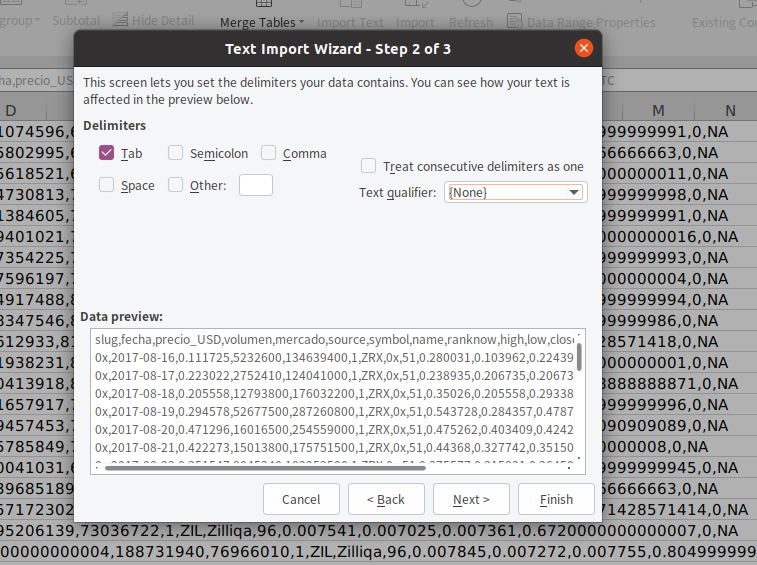
\includegraphics{imagenes/delimitador_incorrecto.png}
\caption{Imagen 1. Delimitador o separador incorrecto: los datos se presentan de forma condensada y desordenada}
\end{figure}

En ese caso, debe intentarse con cada alternativa de delimitador hasta encontrar el que organice los datos de forma correcta. Ese es el delimitador usado para crear el archivo csv.

\begin{figure}
\centering
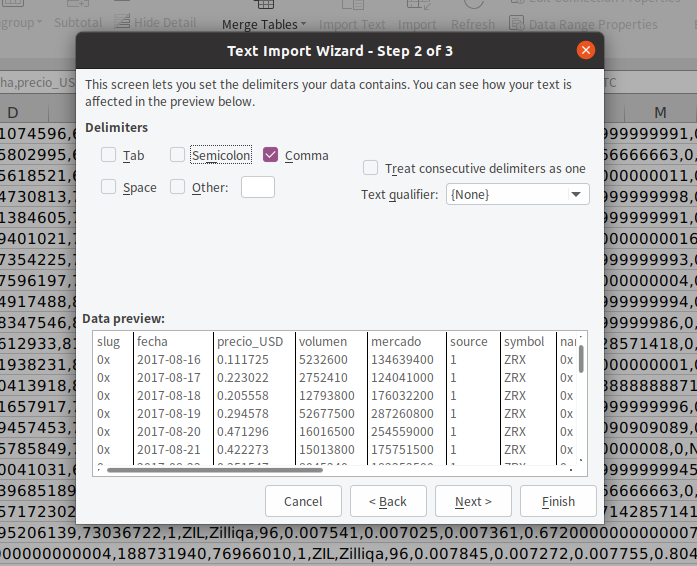
\includegraphics{imagenes/delimitador_correcto.png}
\caption{Imagen 2. Delimitador o separador correcto: los datos se presentan de forma distribuida en celdas y ordenados}
\end{figure}

Conociendo el delimitador, ya se puede cargar el archivo para hacer la verificación de integridad. Para ello debe ejecutarse el siguiente comando:

\begin{Shaded}
\begin{Highlighting}[]
\CommentTok{\# Función 1: carga del archivo con el paquete usado en el script }

\SpecialCharTok{\textless{}}\NormalTok{bbdd}\SpecialCharTok{\textgreater{}} \ErrorTok{\textless{}}\SpecialCharTok{{-}}\NormalTok{ readr}\SpecialCharTok{::}\FunctionTok{read\_delim}\NormalTok{(}\StringTok{"\textless{}/ruta/nombredelarchivo.csv\textgreater{}"}\NormalTok{, }\AttributeTok{delim =} \StringTok{"\textless{}delimitador\textgreater{}"}\NormalTok{, }\AttributeTok{locale =} \FunctionTok{locale}\NormalTok{(}\AttributeTok{decimal\_mark =} \StringTok{","}\NormalTok{, }\AttributeTok{grouping\_mark =} \StringTok{"."}\NormalTok{))}
\end{Highlighting}
\end{Shaded}

Si el archivo carga sin arrojar errores, entonces podrá usarse en el proceso de automatización y cargarse desde el diccionario. En caso de que el código anterior arrojase un error, debe probarse con otras librerías y luego guardarse en formato rds.

El código para la lectura por otra liberaría es el siguiente:

\begin{Shaded}
\begin{Highlighting}[]
\CommentTok{\# Función 2: carga del archivo con otros paquetes}

\SpecialCharTok{\textless{}}\NormalTok{bbdd}\SpecialCharTok{\textgreater{}} \ErrorTok{\textless{}}\SpecialCharTok{{-}}\NormalTok{ data.table}\SpecialCharTok{::}\FunctionTok{fread}\NormalTok{(}\SpecialCharTok{\textless{}}\ErrorTok{/}\NormalTok{ruta}\SpecialCharTok{/}\NormalTok{nombredelarchivo.csv}\SpecialCharTok{\textgreater{}}\StringTok{", sep = "}\SpecialCharTok{\textless{}}\NormalTok{delimitador}\SpecialCharTok{\textgreater{}}\StringTok{", dec="}\SpecialCharTok{\textless{}}\NormalTok{caracter que se usa como separador decimal}\SpecialCharTok{\textgreater{}}\StringTok{")}
\end{Highlighting}
\end{Shaded}

Si la carga con esta librería también arrojase error, debe intentarse con la función que trae la base de R. Para ello debe ejecutarse el siguiente comando:

\begin{Shaded}
\begin{Highlighting}[]
\CommentTok{\# Función 3: carga del archivo con la base}

\SpecialCharTok{\textless{}}\NormalTok{bbdd}\SpecialCharTok{\textgreater{}} \ErrorTok{\textless{}}\SpecialCharTok{{-}} \FunctionTok{read.delim}\NormalTok{(}\StringTok{"\textless{}/ruta/nombredelarchivo.csv\textgreater{}"}\NormalTok{, }\AttributeTok{delim =} \StringTok{"\textless{}delimitador\textgreater{}"}\NormalTok{)}
\end{Highlighting}
\end{Shaded}

Si con cualquiera de las funciones posteriores a la 1 se puede leer el archivo, entonces debe exportarse como rds para que el diccionario llame a este archivo convertido.

Si falla la carga del archivo también con esta última función, dos medidas deben tomarse. La primera es revisar el archivo manualmente y comprobar que los datos estén correctos y que la base de datos haya sido limpiada como se indica en el acápite siguiente de este capítulo. Si aún así persisten los errores, entonces sólo queda gestionar el archivo de nuevo con la fuente administrativa. Para más detalles, véase el diagrama de flujo del proceso de automatización de la producción estadística de SPyJ en el \protect\hyperlink{anexo3}{Anexo 3}

Recuérdese que, como se mencionó en el \protect\hyperlink{formatos_manual}{capítulo 2}, si en cualquiera de estos casos el error consistió en que no se encontró la librería o el paquete, entonces debe instalarse y repetirse la operación. El nombre del paquete con el que se realiza o ejecuta la función es el que está antes de los dos puntos seguidos dobles (::) de la siguiente forma: ::(). En consecuencia, para instalar el paquete debe ejecutarse la siguiente función:

\begin{Shaded}
\begin{Highlighting}[]
\CommentTok{\# Instalar paquete que falta}

\FunctionTok{install.packages}\NormalTok{(}\StringTok{"\textless{}nombredepaquete\textgreater{}"}\NormalTok{)}
\end{Highlighting}
\end{Shaded}

\hypertarget{archivos-en-xlsx}{%
\subsubsection{Archivos en xlsx}\label{archivos-en-xlsx}}

Para verificar la integridad de los archivos remitidos en formato xlsx recuérdese que \textbf{cada base de datos debe ser guardada en un archivo independiente de Excel, que debe contener una única hoja}, la de la base de datos en cuestión. Si el archivo Excel contiene más de una hoja, las funciones siguientes sólo cargarán la primera.

La carga de las bases de datos que se encuentren en Excel se realiza con la siguiente función:

\begin{Shaded}
\begin{Highlighting}[]
\CommentTok{\# Función 1: carga del archivo con el paquete usado en el script }

\SpecialCharTok{\textless{}}\NormalTok{bbdd}\SpecialCharTok{\textgreater{}} \ErrorTok{\textless{}}\SpecialCharTok{{-}}\NormalTok{ openxlsx}\SpecialCharTok{::}\FunctionTok{read.xlsx}\NormalTok{(}\StringTok{"\textless{}/ruta/nombredelarchivo.xlsx\textgreater{}"}\NormalTok{,  }\AttributeTok{detectDates =} \ConstantTok{TRUE}\NormalTok{)}
\end{Highlighting}
\end{Shaded}

Si la función anterior arroja error, entonces debe intentarse con la siguiente:

\begin{Shaded}
\begin{Highlighting}[]
\CommentTok{\# Función 2: carga del archivo con otros paquetes}

\SpecialCharTok{\textless{}}\NormalTok{bbdd}\SpecialCharTok{\textgreater{}} \ErrorTok{\textless{}}\SpecialCharTok{{-}}\NormalTok{ readxl}\SpecialCharTok{::}\FunctionTok{read\_xlsx}\NormalTok{(}\StringTok{"\textless{}/ruta/nombredelarchivo.xlsx\textgreater{}"}\NormalTok{)}
\end{Highlighting}
\end{Shaded}

Si con cualquiera de las funciones posteriores a la 1 se puede leer el archivo, entonces debe exportarse como rds para que el diccionario llame a este archivo convertido.

Si falla la carga del archivo también con esta última función, dos medidas deben tomarse. La primera es revisar el archivo manualmente y comprobar que los datos estén correctos y que la base de datos haya sido limpiada y ajustada como se indica en el acápite siguiente de este capítulo. Si aún así persisten los errores, entonces sólo queda gestionar el archivo de nuevo con la fuente administrativa (\protect\hyperlink{anexo3}{Anexo 3}).

\hypertarget{rds}{%
\subsubsection{Archivos en RDS}\label{rds}}

Si el archivo que se va usar para generar tabulados y/o validar con el script se encuentra en formato rds, implica que R debiera poder leerlo sin inconvenientes. Sin embargo, para evitar problemas posteriores, se recomienda también determinar si carga o no. Para ello, debe ejecutarse el siguiente código:

\begin{Shaded}
\begin{Highlighting}[]
\CommentTok{\# Función 1: carga del archivo en formato rds }

\SpecialCharTok{\textless{}}\NormalTok{bbdd}\SpecialCharTok{\textgreater{}} \ErrorTok{\textless{}}\SpecialCharTok{{-}} \FunctionTok{readRDS}\NormalTok{(}\StringTok{"\textless{}/ruta/nombredelarchivo.rds\textgreater{}"}\NormalTok{)}
\end{Highlighting}
\end{Shaded}

Para guardar una base de datos en formato rds, el comando es el siguiente:

\begin{Shaded}
\begin{Highlighting}[]
\CommentTok{\# Guardar archivo en rds}

\FunctionTok{saveRDS}\NormalTok{(}\SpecialCharTok{\textless{}}\NormalTok{bbdd}\SpecialCharTok{\textgreater{}}\NormalTok{, }\StringTok{"\textless{}/ruta/nombredelarchivo.rds\textgreater{}"}\NormalTok{)}
\end{Highlighting}
\end{Shaded}

\hypertarget{quuxe9-observar-al-realizar-la-verificaciuxf3n-de-integridad}{%
\subsection{¿Qué observar al realizar la verificación de integridad?}\label{quuxe9-observar-al-realizar-la-verificaciuxf3n-de-integridad}}

La verificación de integridad entrega dos resultados:

\begin{enumerate}
\def\labelenumi{\arabic{enumi}.}
\item
  La posibilidad de lectura de las bases de datos por parte de R;
\item
  La lectura correcta de los datos por parte de R.
\end{enumerate}

Los indicadores para determinar si los objetivos de la verificación se cumplen son los siguientes:

\begin{enumerate}
\def\labelenumi{\arabic{enumi}.}
\item
  Que el archivo pueda ser cargado sin errores por R. En algunos casos el proceso de carga puede arrojar advertencias (\emph{warnings}). En principio, no importan. Para la verificación de integridad es relevante sólo si el archivo se carga sin errores. Si en RStudio aparece el objeto con los datos en el panel del entorno global (\emph{Global Enviroment}) y no existe ningún mensaje de error en la consola, entonces se ha cargado correctamente. Puede ser relevante tomar nota de las advertencias (\emph{warnings}), pero que existan no afecta en nada a la verificación. Sólo la presencia o ausencia de mensajes de error son relevantes para determinar la integridad.
\item
  Que los tipos de dato de cada variable del objeto que contiene la base de datos se correspondan con el tipo de dato que se supone debiera contener, especialmente si el tipo ha sido definido en el proceso de limpieza descrito en la siguiente sección del capítulo. Correspondencia del tipo de datos supone que los datos numéricos sean leídos como numéricos (``numeric'' o ``integer''), los de cadena como caracter (chr), y así sucesivamente. Si alguna variable se carga en R como lista (list), entonces hay un error de lectura en los datos y el script no va a poder leer y procesar esa base de datos. Además, especialmente sensibles son los datos que contienen fechas completas (año, mes y día). R tiene que leerlas como fecha (no como número) y en el formato específico usado en automatización siguiendo el estándar ISO 8601: año-mes-día. De lo contrario, hay un error en la lectura de datos de esa variable que debe corregirse manualmente.
\end{enumerate}

Para determinar qué tipos de datos contiene cada variable o columna del objeto con la base de datos, debe ejecutarse la siguiente función:

\begin{Shaded}
\begin{Highlighting}[]
\CommentTok{\# Corroborar los tipos y formatos de datos}

\FunctionTok{str}\NormalTok{(}\SpecialCharTok{\textless{}}\NormalTok{bbdd}\SpecialCharTok{\textgreater{}}\NormalTok{)}
\end{Highlighting}
\end{Shaded}

Si no se cumple alguna de las condiciones mencionadas, entonces la base de datos no ha pasado la verficación y deben hacerse ajustes. Para el indicador 1, ya se ha indicado qué procedimiento debe seguirse. Para el indicador 2, deben ajustarse manualmente los archivos de las bases de datos siguiendo los procedimientos que se indican a continuación, en la segunda parte de este capítulo.

\begin{center}\rule{0.5\linewidth}{0.5pt}\end{center}

\hypertarget{el-ajuste-de-la-estructura-y-los-tipos-de-informaciuxf3n-de-las-bases-de-datos}{%
\section{El ajuste de la estructura y los tipos de información de las bases de datos}\label{el-ajuste-de-la-estructura-y-los-tipos-de-informaciuxf3n-de-las-bases-de-datos}}

Como se mencionaba, cada fuente administrativa remite sus bases de datos con formatos y estructuras propias. Eso exige realizar intervenciones manuales en los archivos respectivos para estandarizarlas. Estandarizadas pueden ser procesadas por los \emph{script}.

Al igual que la verificación de integridad, el ajuste y las modificaciones de las bases de datos son un requisito ineludible: no se pueden usar con los \emph{scripts} de automatización las que no han pasado por este proceso. En todos los casos, dichas modificaciones debe realizarse siguiendo estrictamente y al pie de la letra las siguientes instrucciones.

Para que las instrucciones de este manual sean más comprensibles, se explicaron primero los formatos de archivos de las bases de datos. Sin embargo, se recomienda partir por el proceso de ajuste manual de las bases de datos antes de hacer la verificación de integridad. El flujo de trabajo es más eficiente si la verificación de integridad se realiza en archivos ya estandarizados.

\hypertarget{la-limpieza-de-la-base-de-datos}{%
\subsection{La limpieza de la base de datos}\label{la-limpieza-de-la-base-de-datos}}

La primera operación de estandarización es la limpieza de los archivos de cada base de datos. La limpieza consiste en tres operaciones: i) dejar en el archivo sólo las filas y las columnas necesarias para el procesamiento; ii) modificar los nombres de las columnas para que coincidan con las que los \emph{scripts} van a procesar; y iii) eliminar ``impurezas'' en los datos que pueden alterar el procesamiento por parte de los \emph{scripts}, en particular la ``impureza'' de los espacios en blanco antes o después del contenido de cada dato.

Todas las operaciones deben hacerse siguiendo los siguientes criterios:

\hypertarget{primeras-filas}{%
\subsubsection{Primeras filas}\label{primeras-filas}}

\textbf{La primera fila de cualquier base de datos debe ser la fila que contiene el nombre de las variables o columnas}. Cualquier otra primera fila generará un error en la ejecución de los \emph{scripts} de automatización. Por ello, las filas que estén por encima de la fila del nombre de las columnas o variables, deben ser eliminadas.

Aunque las bases de datos con primeras filas distintas a los nombres de las columnas o variables son comunes en todas las fuentes administrativas, son especialmente frecuentes en los archivos que provienen de la Corporación Administrativa del Poder Judicial. En ellos debe tenerse especial precaución al respecto.

\hypertarget{segundas-filas}{%
\subsubsection{Segundas filas}\label{segundas-filas}}

Las segundas filas de todas las bases de datos deben corresponder al primer registro de datos. No pueden estar compuestas por otros títulos, subtítulos o nombres de variables.

\hypertarget{celdas-combinadas}{%
\subsubsection{Celdas combinadas}\label{celdas-combinadas}}

Ninguna base de datos puede contener celdas combinadas. Su presencia en algún archivo ingresado en el proceso de automatización arrojará error.

\hypertarget{filas-de-totales}{%
\subsubsection{Filas de totales}\label{filas-de-totales}}

Otras filas que deben ser eliminadas de las bases de datos son las filas con la suma de los totales. Si quedan en las bases de datos, generarán una distorsión en los valores procesados por los \emph{scripts}, que arrojará tabulados con resultados incorrectos.

\hypertarget{limpieza-de-columnas-o-variables}{%
\subsubsection{Limpieza de columnas o variables}\label{limpieza-de-columnas-o-variables}}

Las bases de datos que llegan de las fuentes administrativas traen columnas o variables que no son necesarias para que los \emph{scripts} genere los tabulados y la validación. Para reducir los tiempos de carga de bases de datos, consumo de memoria RAM y espacio de almacenamiento en disco, lo recomendable es eliminarlas. Dejarlas en el archivo no afectará mayormente al resultado del procesamiento automatizado, pero para la eventualidad de computadores con bajo rendimiento, lo recomendable es reducir el tamaño de las bases de datos al mínimo necesario.

Las columnas necesarias para ejecutar cada \emph{script} se detallan en el \protect\hyperlink{anexo1}{Anexo 1} para todas y cada una de las bases de datos que se requieren para producir los tabulados y las validaciones de los productos de la Unidad de Seguridad Pública y Justicia

\hypertarget{los-nombres-de-las-variables}{%
\subsubsection{Los nombres de las variables}\label{los-nombres-de-las-variables}}

Cada fuente administrativa remite bases de datos con nombres de variables definidas para su sistemas de administración y gestión de información. Dichos nombres, aunque remitan a una misma variable, son distintos entre la bases de datos de cada fuente administrativa. En algunos caso, incluso una misma fuente administrativa remite dos bases de datos que contienen la misma variable pero con nombres distintos.

Para impedir que esto represente un problema en el procesamiento automatizado de las bases de datos, se requieren la estandarización de nombres de variables. Los nombres de las variables de cada base de datos están especificados en el \protect\hyperlink{anexo1}{Anexo 1}. Deben copiarse en los archivos de las bases de datos tal y como están escritos en dicho anexo. Además, es recomendable, aunque no requisito ineludible, mantener el orden de las variables que se muestra en el anexo, lo que supone mover columnas en los archivos de las bases de datos respectivos.

Deben respetarse las siguientes reglas generales de nombres de variables o columnas:

\begin{itemize}
\item
  los nombres deben escribirse siempre en minúscula;
\item
  los nombres no pueden contener ningún otro carácter que no sea una letra, un número o un guión bajo;
\item
  los espacios deben ser sustituidos por guiones bajos;
\item
  los de las variables que se encuentran detallados en el anexo 1 han sido elegidos en base a estos criterios: que puedan ser uniformes en todas las bases de datos en las que se encuentran y que además sean significativos y autoevidentes, es decir, que cualquiera que esté familiarizado con los cuadros o con las bases de datos pueda interpretar su significado. Es fundamental mantener estos criterios en el caso de incorporar nuevas variables al proceso de generación de cuadros.
\end{itemize}

\hypertarget{eliminaciuxf3n-de-espacios-en-blanco}{%
\subsubsection{Eliminación de espacios en blanco}\label{eliminaciuxf3n-de-espacios-en-blanco}}

Uno de los principales problemas con los que debe lidiar el procesamiento automatizado de bases de datos que no han sido generadas con fines estadísticos es el de la limpieza de cada dato. Cuando los sistemas de gestión no han sido diseñados pensando en criterios estadísticos, los valores se guardan como cadenas que deben ser introducidas por cada usuario del sistema. Y eso es fuente de errores importantes. El más fundamental es registrar información para un mismo valor pero con distintos formato de registros. Por ejemplo, en una misma variable de una misma base de datos se registran de dos formas distintas una región: como ``Región Metropolitana'' o como ``Región Metropolitana de Santiago''.

Todas las bases de datos de los Registros Administrativos que se procesan en la Unidad de Seguridad Pública y Justicia están plagadas de estos errores y problemas de limpieza de información. En algunos casos hay más problemas que en otros, pero todas las bases los presentan.

Como se indica en el \textbf{Manual de Protocolos de Automatización}, la única forma de evitar estos problemas es con bases de datos que registran códigos y se acompañan de un libro de códigos o diccionario de variables. Pero eso supone diseñar los sistemas de gestión y registro de información administrativa para que almacene códigos y no cadenas o caracteres. Con los registros administrativos con los que trabajan la unidad, eso ya no fue posible. Por lo tanto, Sólo queda hacer limpieza de las bases a posteriori.

Parte importante de la limpieza se hace a través de el código de los \emph{scripts}. Sin embargo, hay algunos problemas que son más difíciles de detectar y que requieren funciones complejas para que puedan ser identificados y resueltos. El principal es la existencia de espacios en blanco antes o después de un dato. Este problema es significativo porque altera el tipo de dato: un dato numérico que tiene un espacio antes o después del número genera errores de procesamiento en cualquier lenguaje de programación o software estadístico.

La mejor forma de evitar esto es eliminando esos espacios en blanco previos o posteriores a los datos antes de ingresar la base al proceso de automatización. El último paso, por lo tanto, de la limpieza de bases de datos consiste en eliminar estos caracteres de espacios. Para ello debe usarse la función \texttt{=ESPACIO(\textless{}celda\textgreater{})} de Excel en todos los archivos que se puedan leer desde este programa.

\hypertarget{los-tipos-de-informaciuxf3n-de-las-celdas}{%
\subsection{Los tipos de información de las celdas}\label{los-tipos-de-informaciuxf3n-de-las-celdas}}

La segunda operación de ajuste de las bases de datos consiste en definir explícitamente los tipos de datos que contiene cada columna. En términos estrictos, R interpreta los datos que carga de forma bastante eficaz. Sin embargo, la sola existencia de un dato discordante con el resto en una columna hará que R clasifique de forma distinta a la esperada a la información de toda esa columna. Por ello, debe realizarse esta operación de explicitación del tipo de dato al menos la primera vez que se interviene una base de datos.

\hypertarget{formatos-generales}{%
\subsubsection{Formatos generales}\label{formatos-generales}}

Los formatos se establecen de forma fácil en Excel. Para ello debe abrirse la base de datos, marcar todas las celdas de una columna excepto la del nombre (la primera fila), y elegir el tipo adecuado en el menú ``Formato''.

Importa especialmente definir el formato de los siguientes tipos de datos:

\begin{itemize}
\item
  numéricos;
\item
  cadenas o caracteres;
\item
  fechas
\end{itemize}

\hypertarget{las-fechas}{%
\subsubsection{Las fechas}\label{las-fechas}}

Las fechas son el tipo de dato más delicado debido a que se pueden escribir en múltiples formatos, y la interpretación incorrecta del formato por parte del script genera errores en el procesamiento de la información que detienen la ejecución del código. En el caso de los Registros Administrativos con los que trabaja SPyJ, cada fuente remite la información sobre fechas con el formato que más le acomoda. Muchas veces, dos bases de datos distintas de la misma fuente tiene dos formatos de fecha distintos. Básicamente, las fuentes no tienen criterios definidos ni tampoco mucho cuidado para trabajar las fechas.

Para evitar los problemas que genera la diversidad de formatos, la Organización Internacional para la Estandarización (ISO por su nombre en inglés) ha definido un estándar (ISO 8601) para trabajar con datos sobre fechas que es el que se aplica en el presente sistema de \emph{scripts} y se recomienda respetar en todo proyecto de automatización de estadísticas dentro del INE.

La norma ISO 8601 establece que los datos sobre fechas (o, en términos más generales, sobre temporalidad) deben escribirse en orden descendente, de izquierda a derecha, según el grado de ``amplitud'' de cada componente del dato. En una fecha cualquiera, el año es el valor más amplio, luego le sigue el mes, luego el día, la hora, el minuto y el segundo. El estándar establece que en ese orden deben escribirse los datos de fechas: año-mes-dia. Los datos sobre horas, sin fechas, siguen el mismo criterio de amplitud: hora:minutos:segundos.

Hay otras reglas del estándar además del orden de los datos:

\begin{enumerate}
\def\labelenumi{\arabic{enumi}.}
\item
  El separador de los datos de fecha es el guión;
\item
  El separador de los datos de hora es los dos puntos;
\item
  Si se agrega la hora al dato, se separa de la fecha con la letra T; la media noche del 18 de septiembre de 2021 se escribe de la siguiente forma: 2021-09-18T00:00:00
\item
  También se puede agregar información sobre la zona horaria después de la hora; se escribe con dos caracteres separados por el signo respecto a la hora del meridiano de Greenwich: al oriente, signo positivo; al occidente, signo negativo. Siguiendo el mismo ejemplo anterior, se agrega el huso horario de verano de Chile (tres horas menos que en Greenwich) al 18 de septiembre de 2021 así: 2021-09-18T00:00:00-03:00; el horario de invierno de Chile se muestra así: 2021-09-18T00:00:00-04:00;
\item
  Los años se escriben completos, con cuatro dígitos;
\item
  Todo el resto de los datos se escribe con dos dígitos; los datos para números menores a diez se anteceden de un cero; el 9 de enero de 2021 se escribe así: 2021-01-09;
\end{enumerate}

Al definir el tipo de dato de las variables de fecha en las bases de datos, deben seguirse estos estándares. Para programar el tratamiento de los datos de fechas en los \emph{scripts} no era posible generar código para todos los formatos posibles. Como era necesario adoptar un estándar, se optó por el de ISO. Pero para que funcione, es necesario que en la fase de preparación se convierta las fechas en las bases de dato a este formato.

Esto se puede hacer de forma fácil en Excel siguiendo los mismos pasos descritos en el acápite anterior: se selecciona toda una columna menos la primera y en el menú ``formato de celdas'' se elige ``más formatos de números''. En el cuadro de diálogo se elige ``Fecha'' y en las alternativas se escoge el formato que se ajusta al estándar ISO 8601.

\begin{figure}
\centering
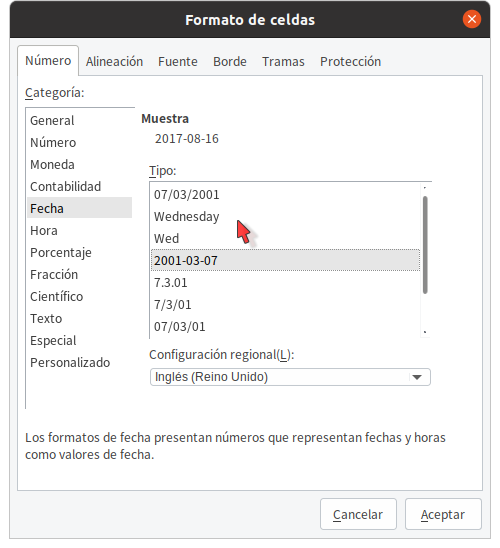
\includegraphics{imagenes/Fecha.png}
\caption{Imagen 3. Definiendo formato de fechas en Excel}
\end{figure}

Por regla general, los archivos exportados a csv automáticamente ajustan el formato de fecha a ISO 8601. De todas formas, debe detectarse si las variables que correspondan tienen el formato correcto en la verificación de integridad. En caso de que eso no ocurra, debe ajustarse el formato. Si la variable contiene sólo fechas, debe aplicarse la siguiente función:

\begin{Shaded}
\begin{Highlighting}[]
\CommentTok{\# Cambiar formato de fecha}

\SpecialCharTok{\textless{}}\NormalTok{bbdd}\SpecialCharTok{\textgreater{}}\ErrorTok{$\textless{}}\NormalTok{variable de fecha}\SpecialCharTok{\textgreater{}} \ErrorTok{\textless{}}\SpecialCharTok{{-}}\NormalTok{ lubridate}\SpecialCharTok{::}\FunctionTok{ymd}\NormalTok{(}\SpecialCharTok{\textless{}}\NormalTok{bbdd}\SpecialCharTok{\textgreater{}}\ErrorTok{$\textless{}}\NormalTok{variable de fecha}\SpecialCharTok{\textgreater{}}\NormalTok{, }\AttributeTok{sep =} \StringTok{"{-}"}\NormalTok{)}
\end{Highlighting}
\end{Shaded}

Si la variable contiene fecha y hora, se aplica la siguiente función:

\begin{Shaded}
\begin{Highlighting}[]
\CommentTok{\# Cambiar formato de fecha y hora}

\SpecialCharTok{\textless{}}\NormalTok{bbdd}\SpecialCharTok{\textgreater{}}\ErrorTok{$\textless{}}\NormalTok{variable de fecha}\SpecialCharTok{\textgreater{}} \ErrorTok{\textless{}}\SpecialCharTok{{-}}\NormalTok{ lubridate}\SpecialCharTok{::}\FunctionTok{ymd\_hms}\NormalTok{(}\SpecialCharTok{\textless{}}\NormalTok{bbdd}\SpecialCharTok{\textgreater{}}\ErrorTok{$\textless{}}\NormalTok{variable de fecha}\SpecialCharTok{\textgreater{}}\NormalTok{, }\AttributeTok{sep =} \StringTok{"{-}"}\NormalTok{)}
\end{Highlighting}
\end{Shaded}

Luego debe exportarse/guardarse el objeto que contiene la base de datos como un archivo rds. Véase las instrucción de la sección \protect\hyperlink{rds}{sección anterior} para ello.

\begin{center}\rule{0.5\linewidth}{0.5pt}\end{center}

\hypertarget{unificaciuxf3n-de-bases-de-datos-divididas-en-muxfaltiples-archivos}{%
\section{Unificación de bases de datos divididas en múltiples archivos}\label{unificaciuxf3n-de-bases-de-datos-divididas-en-muxfaltiples-archivos}}

Una situación frecuente en las bases de datos de Registros Administrativos es que las fuentes remitan la información dividida en varios archivos. El motivo de esto es que Excel, en sus versiones más recientes, puede procesar y contener hasta un máximo de 1.000.000 de filas aprox. Las bases de datos que contenga más de 1.000.000 de casos, entonces, no pueden ser almacenadas en un archivo de Excel en formato xlsx. La solución por parte de la fuente administrativa, por tanto, es remitir la información dividida en varios archivos de Excel.

Los \emph{scripts} de automatización no puede procesar bases de datos divididas en varios archivos. Por lo tanto, se requiere unificarlos en un único archivo. Hay varias alternativas manuales para hacer esto a través de Excel. La más simple es crear un libro, guardarlo en formato binario (xlsb), luego copiar y pegar los datos en la primera hoja y luego guardarlo como archivo csv.

Para evitar hacer esto de forma manual, en el sistema de \emph{scripts} se ha incluido una función que hace la misma operación de forma automatizada. Para que se ejecute correctamente, deben seguirse los siguientes pasos:

\begin{enumerate}
\def\labelenumi{\arabic{enumi}.}
\item
  Limpiar y estandarizar todos y cada uno de los archivos en que se divide la base de datos siguiendo las instrucciones de este capítulo; si sólo se estandarizan y limpian algunos y no todos, o si no se interviene ninguno, la función podría arrojar error; si no todos tienen los mismos nombres de columnas/variables, definitivamente va a arrojar un error.
\item
  Todos los archivos deben guardarse en formato xslx;
\item
  Todos los archivos deben ser puestos en una carpeta en la que se encuentren únicamente los que forman parte de la base de datos; si hay otro archivo en la carpeta que no se corresponda con la base de datos, la función arrojará error.
\item
  Cargar en R las funciones del script de automatización; para ello, deben seguirse las instrucciones del \protect\hyperlink{estructura}{capítulo respectivo}.
\end{enumerate}

Cuando se encuentren todos los archivos en la carpeta y las funciones cargadas, debe ejecutarse la siguiente función:

\begin{Shaded}
\begin{Highlighting}[]
\CommentTok{\# Unificar archivos}

\FunctionTok{unificar\_archivos}\NormalTok{(}\StringTok{"\textless{}ruta/al/directorio\textgreater{}"}\NormalTok{, }\SpecialCharTok{\textless{}}\NormalTok{institución}\SpecialCharTok{\textgreater{}}\NormalTok{, }\SpecialCharTok{\textless{}}\NormalTok{bbdd}\SpecialCharTok{\textgreater{}}\NormalTok{, }\AttributeTok{output =} \StringTok{"\textless{}formato\textgreater{}"}\NormalTok{)}

\CommentTok{\# Ejemplo para unificar archivos de competencia civil guardados en mis documentos}
\CommentTok{\# y exportados en rds:}

\FunctionTok{unificar\_archivos}\NormalTok{(}\StringTok{"\textasciitilde{}/Mis Documentos/"}\NormalTok{, }\StringTok{"pjud"}\NormalTok{, }\StringTok{"terminadas\_civil"}\NormalTok{, }\AttributeTok{output =} \StringTok{"rds"}\NormalTok{)}
\end{Highlighting}
\end{Shaded}

Todos los argumentos son obligatorios.

La función admite sólo dos formatos de salida (output): rds y csv. Cualquier otro formato, arrojará error.

El resultado de la ejecución es un archivo en la misma carpeta de donde tomó los que unió. Tendrá el siguiente nombre: \texttt{\textless{}bbdd\textgreater{}\_\textless{}institución\textgreater{}.\textless{}formato\textgreater{}}. El del ejemplo será el siguiente: \texttt{terminadas\_civil\_pjud.rds}

\hypertarget{el-diccionario}{%
\chapter{El diccionario}\label{el-diccionario}}

El segundo gran insumo para la ejecutar la automatización a través del sistema de \emph{scripts} es el diccionario. Como se había mencionado, el diccionario es un archivo de Excel que contiene las instrucciones necesarias para cargar los archivos que se usan para generar los tabulados y validaciones, la información para controlar el flujo de ejecución del script y, en gran medida, la información auxiliar no contenida en las bases de datos que se utiliza para la tabulación, fundamentalmente categorías de variables complejas, los títulos y las notas a pie de los cuadros.

El uso del diccionario permite controlar la ejecución de algunas operaciones realizadas por los \emph{scripts} sin tener que intervenir el código en R. En otros términos, gracias al diccionario, para controlar un código complejo y escrito en un lenguaje de programación avanzado, se necesita sólo conocimientos de Excel.

Además, el diccionario permite actualizar información sin necesidad de tocar el código de los \emph{scripts}. Por ejemplo, si cambia la familia de algún delito del CUM de un año a otro, para que ese cambio se refleje en los nuevos tabulados, basta con actualizarlo en la hoja de cálculo respectiva del diccionario y no intervenir el código.

Para poder replicar tabulados de cualquier año que se desee y tener siempre acceso a la serie temporal, es recomendable y deseable que se genere un diccionario distinto e independiente para cada año que se generen tabulados automatizados.

Para el correcto funcionamiento de los \emph{scripts}, el contenido del diccionario debe ser tan preciso como las modificaciones manuales que se introducen a las bases de datos. Por lo tanto, es fundamental construir o actualizar este archivo siguiendo de forma estricta las instrucciones contenidas en este capítulo.

\hypertarget{visiuxf3n-general-del-diccionario}{%
\section{Visión general del diccionario}\label{visiuxf3n-general-del-diccionario}}

El diccionario puede estar compuesto por tantas hojas como sean necesarias para generar los tabulados. Pero seis al menos se requieren para cualquiera de las tres fuentes administrativas (PDI, CCH y CAPJ/PJUD) cuyos tabulados son generados por los \emph{scripts}. Son las siguientes:

\begin{itemize}
\item
  La hoja ``meta'';
\item
  La hoja de regiones;
\item
  La hoja de delitos;
\item
  La hoja con el listado de familias de delitos;
\item
  Las hojas con títulos;
\item
  Las hojas con notas a pie.
\end{itemize}

Adicionalmente, en el diccionario se ingresan los datos para la construcción de tabulados con series de tiempo. Más adelante se detalla el procedimiento para esto. Mientras tanto, tómese en consideración que si los tabulados contienen cuadros con series de tiempo, se agrega una hoja de cálculo al diccionario por cada uno de esos cuadros.

A grandes rasgos, este es el diccionario básico: las seis hojas de cálculo mencionadas más las que correspondan a cuadros con series temporales. Con este diccionario básico es posible generar el tabulado más sencillo de los tres: el de PDI.

Para generar el tabulado de Carabineros de Chile, al diccionario básico deben agregarse las siguientes hojas de cálculo:

\begin{itemize}
\item
  La hoja de provincias;
\item
  La hoja de accidentes;
\end{itemize}

Para generar el tabulado de estadísticas judiciales, al diccionario básico debe agregarse la hoja de cálculo con el listado de Cortes de Apelaciones.

A continuación se describen en qué consisten cada una de estas hojas y cómo se construyen.

\hypertarget{la-hoja-meta}{%
\section{La hoja ``meta''}\label{la-hoja-meta}}

La primera hoja, la hoja ``meta'', es la que contiene la información fundamental para la carga de datos por parte de los \emph{scripts} y el control de su flujo. En otros términos, tiene la ``meta-información'' necesaria para que el código procese los datos de las bases y genere los tabulados y las validaciones.

Está compuesta por 6 columnas y, en el estado actual (diciembre de 2020) de las bases de datos, 38 filas sin contar la primera, que contiene los nombres de las columnas. La sexta columna tiene instrucciones sobre cómo llenar la quinta columna, llamada ``cont'', que es una abreviación de ``contenido''. La única de las columnas que debe modificarse y manipularse para controlar el comportamiento de los \emph{scripts} es ésta, la quinta. Las cuatro primeras deben mantenerse intactas, pues de la lectura de su contenido el código obtiene la información para ejecutar operaciones. Si se altera algo de esas columnas, los \emph{scripts} podría romperse o comportarse de forma errática.

La hoja meta debe contener al menos la siguiente información:

\begin{itemize}
\item
  año para el cual se generan los tabulados y/o validaciones;
\item
  ubicación de cada una de las bases de datos necesarias para generar el tabulado de una fuente administrativa;
\item
  ubicación de los archivos validadores;
\item
  el texto que se incorpora como fuente en cada tabulado;
\item
  instrucción para realizar o evitar los tabulados de cada fuente.
\end{itemize}

A continuación se detalla en qué consiste cada tipo de meta-información contenida en la hoja y cómo debe modificarse y administrarse para controlar el comportamiento del script.

\hypertarget{el-auxf1o}{%
\subsection{El año}\label{el-auxf1o}}

Con el id ``agno'', esta meta-información le informa a los \emph{scripts} cuál es el año al que corresponden las bases de datos que va a procesar. Con esa información, crea datos para cuadros con series temporales, nombres de archivos, listas y otros objetos necesarios para la ejecución del código.

Si no se incluye el año en la columna ``cont'', el script arrojará error.

\hypertarget{la-ubicaciuxf3n-de-las-bases-de-datos}{%
\subsection{La ubicación de las bases de datos}\label{la-ubicaciuxf3n-de-las-bases-de-datos}}

La ubicación de las bases de datos se incorpora en la columna ``cont'' para cada fuente administrativa. Se puede identificar qué base de datos se pide en cada fila por el id: un nombre compuesto de al menos dos términos separados por un guión bajo (\_). La última parte del nombre después del último guión bajo identifica a la fuente administrativa: pdi, cch o pjud. Todo lo que se encuentra antes de ese guión bajo corresponde a la base de datos específica para esa fuente. Así, el id ``victimas\_pdi'' refiere a la base de datos ``víctimas'' de la PDI; el id ``suprema\_terminadas\_pjud'' corresponde a la base de datos de causas terminadas en la Corte Suprema.

En la columna ``cont'' debe incluirse la ubicación física del archivo que contiene la base de datos: la ruta completa al directorio y el nombre del archivo, con extensión incluida. Así, si el archivo de la base de datos de causas civiles terminadas se encuentra en el directorio ``bases de datos'' de la unidad principal del computador, el contenido de la columna ``cont'' debiera ser el siguiente: \texttt{c://bases\ de\ datos/civiles\ terminadas.csv}.

Sólo pueden ingresarse rutas a ubicaciones locales, dentro del computador. El script no soporta el ingreso de direcciones remotas de red o web.

En la actualidad (diciembre de 2020), los tabulados completos de las tres fuentes administrativas (44 cuadros de PDI; 40 de Carabineros de Chile y 29 del Poder Judicial) se generan a partir de 27 bases de datos: 4 para PDI, 5 para CCH y 18 para CAPJ/PJUD. Si no desea generarse el tabulado de una fuente en particular, entonces la columna ``cont'' de todas sus bases de datos debe quedar en blanco, sin ningún contenido. Pero si se ingresa la ubicación de al menos una base de datos para esa fuente, deben ingresarse todas. De lo contrario, el código generará error. Ejemplo: si sólo queremos generar los tabulados de PDI, la columna ``cont'' para las bases de datos de las otras dos fuentes (CCH y CAPJ/PJUD) deben quedar vacías; pero además, deben ingresarse las ubicaciones de las cuatro bases de datos de PDI. Si se ingresa la ubicación de tres o menos bases de datos, el código primero arrojará una advertencia y luego un error.

De igual forma, si al menos una de las ubicaciones de las bases de datos ha sido ingresada de forma incorrecta, el script arrojará error.

\hypertarget{ubicaciuxf3n-de-los-archivos-validadores}{%
\subsection{Ubicación de los archivos validadores}\label{ubicaciuxf3n-de-los-archivos-validadores}}

El ingreso de la ubicación de los archivos validadores debe hacerse de la misma forma que se ingresa la ubicación para las bases de datos. En la columna id, los nombres de los validadores tienen como prefijo, precisamente, la palabra ``validadores'' y se encuentra separada del nombre de la fuente administrativa por un guión bajo. La ruta completa, incluida el nombre del archivo y su extensión, debe ingresarse en la columna ``cont'' respectiva.

Si no se desea que los \emph{scripts} realicen una validación de los tabulados de una fuente administrativa específica, la columna ``cont'' respectiva debe quedar vacía, sin ningún contenido. Si, por el contrario, se agrega la ubicación correcta de un archivo para validar (según las instrucciones del próxima capítulo), los \emph{scripts} generará un archivo Excel que mostrará todas las discrepancias que existen entre los cuadros generados de forma atuomatizada, de un lado, y los cuadros contenidos en el archivo validador, del otro.

Si se ingresa una ruta incorrecta, los \emph{scripts} arrojarán un error.

\hypertarget{texto-de-la-fuente-para-tabulados}{%
\subsection{Texto de la fuente para tabulados}\label{texto-de-la-fuente-para-tabulados}}

En la hoja ``meta'' también se ingresa el texto que se adjunta al pie de cada cuadro indicando la fuente de procedencia de los datos. En la columna id, los nombres de las fuentes tienen como prefijo la palabra ``fuente'' y se encuentra separada del nombre de la fuente administrativa por un guión bajo. En la columna ``cont'' debe ingresarse el texto que se desea aparezca en los cuadros respectivos. Por ejemplo: el texto que aparecerá al pie de los cuadros de Carabineros de Chile como fuente debe agregarse en la columna ``cont'' que corresponde a la fila con id ``fuente\_cch''.

\hypertarget{instrucciuxf3n-para-generar-o-evitar-los-tabulados}{%
\subsection{Instrucción para generar o evitar los tabulados}\label{instrucciuxf3n-para-generar-o-evitar-los-tabulados}}

Las últimas filas del archivo contienen controladores de flujo. Se identifican por el prefijo ``procesar'' separado del nombre de la fuente administrativa por un guión bajo. Su función es indicarle al código si genera o no el archivo Excel con los tabulados de la fuente respectiva. Si se escribe cualquier cosa en la columna ``cont'', entonces el código generará el archivo Excel con los tabulados respectivos. Para evitar que genere el archivo, la columna correspondiente debe quedar en blanco.

Si, por ejemplo, se requiere validar los tabulados del Poder Judicial pero no se generar el archivo con los tabulados automatizados, debe ingresarse la ubicación del archivo judicial en la fila con id ``validador\_pjud'' y dejarse en blanco el controlador de flujo para la misma fuente: ``procesar\_pjud''.

Si se dejan en blanco ambos valores y se ingresan todas las bases de datos de la fuente administrativa correspondiente, entonces el script cargará las bases, generará los cuadros, pero no los guardará en el archivo Excel de tabulados ni creará el archivo de validación. Habrá cargado la bases de datos y procesado tabulados de forma innecesaria e ineficiente, sin propósito. Si no se desea procesar ni tabulados ni validación de alguna fuente en particular, deben también dejarse en blanco las columnas ``cont'' correspondientes a las bases de datos.

Si no se ingresan bases de datos para una fuente y, sin embargo, sí se ingresa la ubicación de su validador y/o algún contenido a su controlador de flujo, el script arrojará error.

\hypertarget{control-del-comportamiento-de-los-scripts}{%
\subsection{\texorpdfstring{Control del comportamiento de los \emph{scripts}}{Control del comportamiento de los scripts}}\label{control-del-comportamiento-de-los-scripts}}

Esta es la forma en que se controla el comportamiento y el flujo de los \emph{script}: a través del contenido que se ingresa en la columna ``cont'' de la hoja ``meta''. Si se desea generar tabulados sólo para una fuente (por ejemplo, PDI), las celdas correspondientes a las otras fuentes deben dejarse en blanco. Si sólo se desea generar tabulados de esa fuente, también debe dejarse en blanco la columna ``cont'' de su validador; o viceversa: si sólo se desea validar cuadros sin generar el archivo con el tabulado completo, debe dejarse en blanco la columna ``cont'' de su controlador de flujo (en este caso, ``procesar\_pdi''). Y así sucesivamente.

\hypertarget{la-hoja-de-regiones}{%
\section{La hoja de regiones}\label{la-hoja-de-regiones}}

La segunda hoja de cálculo del diccionario es la que tiene el listado de todas las regiones del país, con sus nombres básicos y también con las posibles combinaciones complejas de sus nombres con prefijos y sufijos. De esta hoja toma el código los nombres de las regiones que se agregan a los cuadros, pero también la información para ordenarlas.

Esta hoja debe mantenerse tal como se encuentra en la actualidad. El único motivo para modificarla sería la creación de una nueva región, que debiera agregarse al final del listado con la información correspondiente.

\hypertarget{la-hoja-de-provincias}{%
\section{La hoja de provincias}\label{la-hoja-de-provincias}}

Es similar a la hoja de regiones. Cumple la misma función, pero contiene el listado de las provincias. Tampoco debe modificarse a menos que se requiera incorporar una nueva provincia.

\hypertarget{la-hoja-con-las-cortes-de-apelaciones}{%
\section{La hoja con las Cortes de Apelaciones}\label{la-hoja-con-las-cortes-de-apelaciones}}

Similar a las hojas de regiones y provincias. Aporta nombres a los cuadros y el orden en el que se desplegarán.

No debe modificarse a menos que existan motivos debidamente fundados.

\hypertarget{la-hoja-de-delitos}{%
\section{La hoja de delitos}\label{la-hoja-de-delitos}}

Contiene un listado de todos los delitos incluidos en el CUM de cada año, con su código, su glosa y la familia a la que pertenecen.

Si de un año a otro se produce una modificación en la forma de registrar un delito, debe incorporarse en esta hoja de cálculo. Ejemplo hipotético: si el delito ``maltrato a persona mayor de edad'', que hoy se agrupa en la familia ``Violencia Intrafamiliar'', pasa a la familia ``Contra las personas'', entonces la modificación respectiva debe hacerse en esta hoja.

\hypertarget{la-hoja-de-familias-de-delitos}{%
\section{La hoja de familias de delitos}\label{la-hoja-de-familias-de-delitos}}

Contiene un listado de las familias de delitos ordenadas de acuerdo a como se presentan en los tabulados publicados. Su función es simplemente aportar el orden de las familia. No debe modificarse a menos que cambie el orden con el que se desea se presenten en los cuadros a publicar.

Si el texto de los nombres de las familias de esta hoja no es idéntico al texto de las familias de la hoja anterior, entonces el script no podrá incluir la familia respectiva en los cuadros con delitos. Es indispensable que no exista discrepancia entre ambas hojas.

\hypertarget{la-hoja-de-accidentes}{%
\section{La hoja de accidentes}\label{la-hoja-de-accidentes}}

Contiene el listado con los nombres de los accidentes registrados por Carabineros de Chile y el orden en que se despliegan. Si se produce un cambio en los nombres o el orden, debe incorporarse en esta hoja para que quede reflejado en los tabulados.

\hypertarget{hojas-con-los-tuxedtulos}{%
\section{Hojas con los títulos}\label{hojas-con-los-tuxedtulos}}

Los títulos de los cuadros se añaden a través del diccionario. Existe una hoja con títulos para cada fuente administrativa. El nombre de cada una de ellas corresponde al prefijo ``titulos'' y se encuentra separada del nombre de la fuente administrativa por un guión bajo. Los títulos de los cuadros del Poder Judicial, por ejemplo, se encuentran en la hoja llamada ``titulos\_pjud''.

Dos columnas tiene cada una de estas hojas: la del número de cuadro y la del texto del título. Para los cuadros que llevan más de un título, deben agregarse todos, uno por línea. Si entre dos títulos existiese una línea en blanco, también debe agregarse en la hoja. Así quedan los títulos de los cuatro primeros cuadros del tabulado de PDI 2019:

\begin{longtable}[]{@{}ll@{}}
\toprule
\begin{minipage}[b]{(\columnwidth - 1\tabcolsep) * \real{0.50}}\raggedright
\emph{cuadro}\strut
\end{minipage} & \begin{minipage}[b]{(\columnwidth - 1\tabcolsep) * \real{0.50}}\raggedright
\emph{titulo}\strut
\end{minipage}\tabularnewline
\midrule
\endhead
\begin{minipage}[t]{(\columnwidth - 1\tabcolsep) * \real{0.50}}\raggedright
1\strut
\end{minipage} & \begin{minipage}[t]{(\columnwidth - 1\tabcolsep) * \real{0.50}}\raggedright
CAPÍTULO I: DELITOS INVESTIGADOS\strut
\end{minipage}\tabularnewline
\begin{minipage}[t]{(\columnwidth - 1\tabcolsep) * \real{0.50}}\raggedright
1\strut
\end{minipage} & \begin{minipage}[t]{(\columnwidth - 1\tabcolsep) * \real{0.50}}\raggedright
\strut
\end{minipage}\tabularnewline
\begin{minipage}[t]{(\columnwidth - 1\tabcolsep) * \real{0.50}}\raggedright
1\strut
\end{minipage} & \begin{minipage}[t]{(\columnwidth - 1\tabcolsep) * \real{0.50}}\raggedright
DELITOS INVESTIGADOS POR FAMILIA DE DELITOS Y MATERIAS\strut
\end{minipage}\tabularnewline
\begin{minipage}[t]{(\columnwidth - 1\tabcolsep) * \real{0.50}}\raggedright
1\strut
\end{minipage} & \begin{minipage}[t]{(\columnwidth - 1\tabcolsep) * \real{0.50}}\raggedright
CUADRO 1: NÚMERO DE DELITOS INVESTIGADOS POR AÑO, SEGÚN REGIÓN\strut
\end{minipage}\tabularnewline
\begin{minipage}[t]{(\columnwidth - 1\tabcolsep) * \real{0.50}}\raggedright
2\strut
\end{minipage} & \begin{minipage}[t]{(\columnwidth - 1\tabcolsep) * \real{0.50}}\raggedright
CUADRO 2: NÚMERO DE DELITOS INVESTIGADOS POR REGIÓN, SEGÚN FAMILIA Y MATERIAS, 2019\strut
\end{minipage}\tabularnewline
\begin{minipage}[t]{(\columnwidth - 1\tabcolsep) * \real{0.50}}\raggedright
3\strut
\end{minipage} & \begin{minipage}[t]{(\columnwidth - 1\tabcolsep) * \real{0.50}}\raggedright
CUADRO 3: NÚMERO DE DELITOS INVESTIGADOS POR MES DE OCURRENCIA, SEGÚN FAMILIA Y MATERIAS, 2019\strut
\end{minipage}\tabularnewline
\begin{minipage}[t]{(\columnwidth - 1\tabcolsep) * \real{0.50}}\raggedright
4\strut
\end{minipage} & \begin{minipage}[t]{(\columnwidth - 1\tabcolsep) * \real{0.50}}\raggedright
CUADRO 4: NÚMERO DE DELITOS INVESTIGADOS POR DÍA DE OCURRENCIA, SEGÚN FAMILIA Y MATERIAS, 2019\strut
\end{minipage}\tabularnewline
\bottomrule
\end{longtable}

Nótese que la segunda fila tiene número de cuadro pero no contenido en la columna del título. Se agregará de esa forma al cuadro que quede en el archivo final del tabulado.

El texto de los títulos será tomado por los \emph{scripts} tal y como se ingrese en esta hoja de cálculo.

\hypertarget{hojas-con-las-notas-al-pie}{%
\section{Hojas con las notas al pie}\label{hojas-con-las-notas-al-pie}}

Las notas al pie se ingresan de la misma forma que los títulos: en hojas específicas para cada fuente administrativa. Se identifican porque el nombre de cada una de ellas corresponde al prefijo ``notas'' y se encuentra separada del nombre de la fuente administrativa por un guión bajo.

La hoja de las notas es más compleja que la de títulos. Requiere información para seis variables:

\begin{itemize}
\item
  cuadro: el número del cuadro al que se agregará la nota;
\item
  fila: número de fila en la que se insertará;
\item
  columna: número de columna; como en Excel las columnas se designan con letras, el número debe calcularse. Cualquiera que sea el método que se elija para ello, este dato debe ingresarse en formato numérico;
\item
  ancla: texto al cual se añadirá el número de la nota; el texto debe estar compuesto por una palabra o número, pero sólo uno/a; el script no soporta insertar el número de nota a otro tipo de texto que no sea una palabra o un número;
\item
  numero: número de la nota para el cuadro al que se agrega;
\item
  texto: el contenido textual de la nota.
\end{itemize}

Para cada nota, todos estos seis valores son obligatorios. Si falta alguno, la nota no se agregará o el código puede arrojar error.

\hypertarget{hojas-con-series-temporales}{%
\section{Hojas con series temporales}\label{hojas-con-series-temporales}}

A través del diccionario también se generan cuadros con series temporales. En lugar de generar el dato para cada año a partir de las bases de datos, cada \emph{script} calcula el valor para el año de referencia y lo une al cuadro que se encuentra en el diccionario.

Para ello, debe pegarse el cuadro con los datos de todos los años anteriores. El script los tomará para unirlo al dato del año de referencia.

Es importante respetar la forma de nombrar la hoja para que el script sepa de donde tomar el dato. El nombre se compone del prefijo ``c'' seguido del número de cuadro del que se trate; como sufijo se usa la fuente administrativa, que se separa del prefijo con un guión bajo. Así, para el generar el cuadro 35 con una serie temporal con datos de Carabineros de Chile, la hoja debe llevar el siguiente nombre: c35\_cch.

\hypertarget{el-archivo-validador}{%
\chapter{El archivo validador}\label{el-archivo-validador}}

El archivo validador es el tercer gran insumo que se genera en la fase de preparación o fase manual de la automatización. A diferencia de los otros dos insumos, las bases de datos y el diccionario, el archivo validador es opcional. Sólo debe generarse en caso de que se desee validar los resultados del procesamiento automatizado. En caso de que no se desee realizar la validación, el código de los \emph{scripts} puede generar los tabulados sin necesidad de que exista este archivo.

El archivo validador contiene los datos que se espera contenga el archivo con los tabulados automatizados. Estos datos pueden provenir de un tabulado manual o de los propios tabulados remitidos por las fuentes administrativas. El requisito es que sirva como una suerte de espejo en el que se va a mirar el archivo con los tabulados generados a través de los \emph{scripts} de automatización. Eso supone que, en el caso de un tabulado automatizado perfecto, serán idénticos los cuadros del archivo validador y los generados por los \emph{scripts}. Si hay al menos una discrepancia, el código generará un archivo de Excel que contenga todos los datos que sean distintos entre un archivo y otro.

Para generar un archivo validador eficaz que no arroje errores y que reduzca al mínimo los falsos positivos, deben seguirse las siguientes instrucciones.

\hypertarget{contenido-y-estructura-del-archivo-validador}{%
\section{Contenido y estructura del archivo validador}\label{contenido-y-estructura-del-archivo-validador}}

El archivo validador está compuesto por la misma cantidad de hojas de cálculo que debe tener el archivo con los tabulados que ha sido generado por el sistema de \emph{scripts} de automatización. Por ejemplo: si el archivo con los tabulados de PDI contiene 44 hojas de cálculo, una por cada cuadro, el archivo validador debe tener esas mismas 44 hojas de cálculo.

Las hojas de cálculo deben ordenarse en la misma secuencia que se espera estén ordenadas en el archivo con el tabulado automatizado. El nombre de cada hoja debe ser el número secuencial; la primera hoja lleva por nombre 1; la segunda lleva por nombre 2; la tercera, 3, y así sucesivamente hasta el cuadro 44 en el caso de PDI.

En cada hoja de cálculo se incluye sólo el cuadro, sin títulos ni notas al pie. Además, deben suprimirse todos los formatos y las fórmulas. La hoja debe contener únicamente nombres de columnas y valores crudos, ya sean textos o números. El código podrá comparar así celda a celda de cuadro a cuadro para identificar discrepancias.

Es fundamental que el archivo validador tenga una única celda de encabezados o nombres de variables/columnas. Todas las celdas combinadas deben eliminarse, y la segunda fila siempre debe ser de datos, nunca de títulos o subtítulos.

\hypertarget{resultado-de-la-validaciuxf3n}{%
\section{Resultado de la validación}\label{resultado-de-la-validaciuxf3n}}

Como se mencionaba, si el código identifica discrepancias entre los cuadros generados por la automatización y los cuadros contenidos en el archivo validador, entonces generará un archivo Excel de una única hoja de cálculo.

Las discrepancias pueden ser de dos tipos. La primera es la que se produce entre cuadros de iguales dimensiones, es decir, entre cuadros que tienen la misma cantidad de columnas y la misma cantidad de filas. En este caso, el proceso de validación compara el contenido celda a celda. El archivo con los resultados de la validación indicará el cuadro, la fila y la columna de la celda en que se produce la discrepancia. En una cuarta columna indicará cuál es el contenido de la celda en el cuadro producido por los \emph{scripts} de automatización, y en la quinta columna indicará cuál es el contenido de la celda del cuadro incluido en el archivo validador.

El segundo tipo de discrepancia se produce cuándo no existe coincidencia de dimensiones entre los cuadros, ya sea porque el del tabulado o el del archivo validador tienen más columnas y/o más filas que el otro. En estos casos, el archivo con el resultado la validación contendrá filas en color rojo identificando el cuadro en el que esto se produce. Dichos cuadros no han sido validados en el sentido estricto de la palabra; o al menos en el sentido descrito en el párrafo anterior: comparación de contenido celda a celda.

Para que se produzca una validación efectiva en caso de este segundo tipo de discrepancia, es necesario corregir o bien el fragmento de código que genera el cuadro dentro del archivo del \emph{script} correspondiente, o bien el cuadro correspondiente en el archivo validador. Luego de la corrección debe repetirse todo el proceso de validación; sólo así el código estará en condiciones de determinar si existen diferencias efectivas en los valores de ambos cuadros. Si las dimensiones son distintas, los \emph{scripts} no pueden hacer una comparación celda a celda.

Este procedimiento de igualación de dimensiones de los cuadros debe replicarse o iterarse cuantas veces sean necesarias hasta eliminar las discrepancias entre números de filas y/o columnas.

\hypertarget{precauciones}{%
\section{Precauciones}\label{precauciones}}

Si bien el proceso de validación es capaz de identificar diferencias estadísticas reales, también es muy sensible a los falsos positivos. En el archivo con el resultado de la validación aparecerán diferencias o discrepancias de todo tipo que no necesariamente implican invalidez o error en los datos estadísticos. Las más comunes de estas diferencias se producen en las celdas con contenido de texto. La diferencia entre una mayúscula y una minúscula, entre una palabra con tilde y una sin tilde, entre una celda que no tiene espacios en blanco antes o después de los datos y otra celda que si los tiene, no son errores estadísticos; sin embargo, aparecerán como discrepancias entre el archivo validador y el tabulado automatizado.

Por lo anterior, para analizar y ponderar las discrepancias, es recomendable filtrar las filas del archivo con los resultados de la validación que contengan sólo datos numéricos.

\hypertarget{part-tercera-parte-estructura-del-sistema-de-scripts}{%
\part*{TERCERA PARTE: ESTRUCTURA DEL SISTEMA DE SCRIPTS}\label{part-tercera-parte-estructura-del-sistema-de-scripts}}
\addcontentsline{toc}{part}{TERCERA PARTE: ESTRUCTURA DEL SISTEMA DE SCRIPTS}

\hypertarget{presentaciuxf3n-de-la-tercera-parte}{%
\chapter*{Presentación de la tercera parte}\label{presentaciuxf3n-de-la-tercera-parte}}
\addcontentsline{toc}{chapter}{Presentación de la tercera parte}

El sistema de \emph{scripts} de automatización se puede ejecutar una vez que ha concluido la fase de preparación y están listos todos los insumos necesarios para la generación de tabulados. La ejecución, sin embargo, puede arrojar errores. Es fundamental, por lo tanto, saber interpretar esos errores, saber dónde y por qué se produjeron y tener una noción de cómo corregirlos. Eso supone un conocimiento básico de la estructura y funcionamiento del script.

Esta tercera parte aporta eso.

\hypertarget{estructura}{%
\chapter{La estructura del script}\label{estructura}}

Como se había mencionado en la introducción, el sistema de \emph{scripts} es un conjunto de archivos que están relacionados entre sí y que se ejecutan de acuerdo a los contenidos en la hoja ``meta'' del diccionario.

El sistema entero está está en una carpeta: Automatización\_SPyJ. Dentro de esa carpeta existen tres subcarpetas y un archivo en particular llamado \texttt{init.R}. El script se ejecuta corriendo las instrucciones contenidas en este archivo.

\hypertarget{el-flujo-de-init.r}{%
\section{El flujo de init.R}\label{el-flujo-de-init.r}}

\texttt{init.R} primero carga los paquetes necesarios para la ejecución del código. Con el objeto de no complejizar innecesariamente los \emph{scripts}, se ha desarrollado su código reduciendo al mínimo posible los paquetes necesarios para ejecutarlo.

En segundo lugar, carga las funciones creadas específicamente para la ejecución de las tareas de los \emph{scripts}. Dichas funciones se encuentran en una subcarpeta llamada ``R'' y están divididas en dos archivos. El primero de ellos, llamado \texttt{específicas.R}, contiene todas las funciones que se han creado para estos \emph{scripts} específicamente y que no necesitan que se cargue previamente el diccionario. El segundo archivo, llamado \texttt{post\_dict.R}, contiene todas las funciones escritas para el script pero que requieren que se cargue previamente el diccionario. Por lo tanto, se llaman después del paso siguiente, que es, precisamente, la carga del diccionario.

La carga del diccionario se realiza a través de una función contenida en el archivo especificas.R: \texttt{ingresar\_diccionario()}. Como argumento, incluye la ruta completa al diccionario, incluidos su nombre y su extensión

\begin{Shaded}
\begin{Highlighting}[]
\CommentTok{\# Cargando el diccionario }

\FunctionTok{ingresar\_diccionario}\NormalTok{(}\StringTok{"/ruta/completa/al/dicionario.xlsx"}\NormalTok{)}
\end{Highlighting}
\end{Shaded}

Mientras no se desarrolle una interfaz gráfica para ingresar la ruta al diccionario, esta es la única intervención que debe hacerse a los archivos del sistema de \emph{scripts} para poder ejecutarlo: escribir la ruta al archivo del diccionario como argumento de la función que lo carga. No hay ninguna otra intervención al código que corresponda o sea necesario hacer para ejecutarlo.

La carga del diccionario no sólo supone que R lea ese archivo. La lectura implica la ejecución de todas las operaciones subsiguientes para preparar la generación de tabulados y/o la realización de validaciones. En otras palabras, la carga del diccionario gatillará automáticamente la carga de las bases de datos, de archivos de validación, de formatos, etc.

\hypertarget{generaciuxf3n-de-tabulados-y-validaciones}{%
\section{Generación de tabulados y validaciones}\label{generaciuxf3n-de-tabulados-y-validaciones}}

Al terminar de cargar el diccionario y ejecutar todas las operaciones que gatilla, init.R ejecuta las instrucciones para generar los cuadros de aquellas fuentes administrativas para las que se cargaron las bases de datos a través del diccionario. Si no se cargaron las bases de datos, entonces no ejecutará el código para crear los cuadros respectivos. Y sin ello, no se genera el archivo con los tabulados ni el archivo con la validación.

En caso de que sí se hayan cargado las bases de datos para una fuente administrativa en específico, \texttt{init.R} llama a un archivo con el código necesario para crear los cuadros de esa fuente. Dicho archivo también se encuentra en la subcarpeta \texttt{R}. Por ejemplo, si a través del diccionario se han cargado las 4 bases de datos de PDI, entonces \texttt{init.R} llamará al archivo con los códigos que generan los cuadros de PDI. Dicho archivo tiene el nombre de \texttt{tabs\_pdi.R}. Y esto aplica como regla general: los nombres de los archivos con el código para generar los cuadros se encuentran en la subcarpeta \texttt{R} y llevan el nombre de ``tabs'' seguido de un guión bajo y de la fuente.

\hypertarget{localizaciuxf3n-de-bugs}{%
\section{Localización de bugs}\label{localizaciuxf3n-de-bugs}}

Mientras se ejecuta el código, en el terminal aparecerán mensajes indicando el estado de avance de la ejecución. En específico, indicará cuál es el último cuadro procesado. Así, si el script arroja algún error, se sabrá en qué parte del código buscarlo y corregirlo: el archivo con el código para tabulados de la fuente respectiva, en el cuadro inmediatamente posterior al último terminado.

Si el error no se localiza en esa parte específica del código, entonces debe buscarse en las funciones que llama los \emph{scripts} para construir el cuadro con el bug.

\hypertarget{ejecuciuxf3n-del-script}{%
\section{Ejecución del script}\label{ejecuciuxf3n-del-script}}

Para esta versión del script, la única forma de ejecutarlo consiste en hacer correr el código del archivo \texttt{init.R}. Para ello, debe abrirse en RStudio y presionar las teclas Ctrl+Alt+R después de ingresar la ruta al diccionario en la función \texttt{ingresar\_diccionario()}.

\hypertarget{part-anexos}{%
\part*{ANEXOS}\label{part-anexos}}
\addcontentsline{toc}{part}{ANEXOS}

\hypertarget{anexo1}{%
\chapter*{Anexo 1: Nombres de variables de bases de datos}\label{anexo1}}
\addcontentsline{toc}{chapter}{Anexo 1: Nombres de variables de bases de datos}

\hypertarget{anexo-2-mejoras-pendientes-al-script-v.-0.1}{%
\chapter*{Anexo 2: Mejoras pendientes al script v. 0.1}\label{anexo-2-mejoras-pendientes-al-script-v.-0.1}}
\addcontentsline{toc}{chapter}{Anexo 2: Mejoras pendientes al script v. 0.1}

\hypertarget{mejoras-planificadas}{%
\section*{Mejoras planificadas}\label{mejoras-planificadas}}
\addcontentsline{toc}{section}{Mejoras planificadas}

\begin{enumerate}
\def\labelenumi{\arabic{enumi}.}
\item
  Crear una ShinyApp para cargar diccionario a través de interfaz gráfica;
\item
  Ampliar código para que pueda iniciarse la ejecución del código a través de cualquiera de las tres alternativas: interfaz gráfica, consola/script o terminal.
\item
  Corregir las materias de la competencia de familia, que en la actualidad están sin texto (glosa) debido a los graves errores que traen las bases de datos.
\item
  Hoja de cálculo con el índice para cada tabulado;
\item
  Ampliar la función de tabulación para que aplique estilos a CCH y PJUD. Ahora los aplica sólo a PDI;
\item
  Corregir con \texttt{regexp} la asignación de formato ``negrita'' a las filas cuando tengan el número de una nota al pie;
\item
  Desarrollar función para que la nota al pie se pegue a pesar de signos de puntuación. Eso se hace con \texttt{regexp};
\item
  Hacer que la nota al pie aparezca en superíndice;
\item
  Arreglar la conformación de los cuadros de nacionalidades (c28 de PDI). Actualmente las nacionalidades en ``otros'' están listada con detalle. Eso implica que si en una próxima versión de los tabulados aparece una persona detenida de una nacionalidad que no aparezca en el listado, no se contabilizará en la categoría ``otras'' y generará un número incorrecto
\item
  Poner negritas a ``Menores'' y ``Adultos'' en c27 de PDI
\item
  Modificar el código de guardado de RDS para que sustituya la extensión del archivo cuando se agregan variables que no estaban (sección limpieza);
\item
  Reducir a función la creación de los objetos de los libros de Excel de la tabulación y validación. En la actualidad están como código repetido al final de cada uno de los archivos .R que generan los tabulados;
\item
  La función anterior debe agregar el año al nombre del tabulado que arroja como resultado. Ej: \texttt{tabulados\_cch\_2020.xlsx}.
\end{enumerate}

\hypertarget{mejoras-a-evaluar}{%
\section*{Mejoras a evaluar}\label{mejoras-a-evaluar}}
\addcontentsline{toc}{section}{Mejoras a evaluar}

\begin{enumerate}
\def\labelenumi{\arabic{enumi}.}
\item
  Cambiar paquete que lee xlsx: openxlsx por readxl. Este último tiene la opción de trim al momento de leer archivos
\item
  Corregir que las tablas incluyan filas que no tengan valores. Se requiere una definición en la Unidad de SPyJ para eso.
\end{enumerate}

\hypertarget{anexo3}{%
\chapter*{Anexo 3: Diagrama de flujo: generación automatizada de tabulados de SPyJ}\label{anexo3}}
\addcontentsline{toc}{chapter}{Anexo 3: Diagrama de flujo: generación automatizada de tabulados de SPyJ}

El sistema de \emph{scripts} para la producción de tabulados de estadísticas de Seguridad Pública y Justicia fue pensado y programado siguiendo el flujo que se encuentra en el siguiente diagrama: https://miro.com/app/board/o9J\_kpazWcw=/

  \bibliography{book.bib}

\end{document}
